\documentclass[a4paper, 14pt]{extarticle}
\usepackage{geometry}

\usepackage{cmap} % Улучшенный поиск русских слов в полученном pdf-файле
\usepackage{mathtext} % русские буквы в формулах
\defaulthyphenchar=127 % Если стоит до fontenc, то переносы не впишутся в выделяемый текст при 
%копировании его в буфер обмена
\usepackage[T2A]{fontenc}
\usepackage[utf8]{inputenc}
\usepackage[english, russian]{babel}
\usepackage{pscyr}  
\renewcommand{\rmdefault}{ftm} % ftm - (TimesNewRoman), fac - Academy, fad - Advertisement, flz - 
%Lazurski, fcr - CourierNewPSM, others in pscyr.sty

\usepackage{amsthm,amsfonts,amsmath,amssymb,amscd} % Математические дополнения от AMS
\usepackage{mathtools} % Добавляет окружение multlined

\usepackage{longtable} % Длинные таблицы
\usepackage{multirow,makecell,array} % Улучшенное форматирование таблиц
\usepackage{booktabs} % Возможность оформления таблиц в классическом книжном стиле

\usepackage{soulutf8} % Поддержка переносоустойчивых подчёркиваний и зачёркиваний
\usepackage{icomma} % Запятая в десятичных дробях

\usepackage[usenames,dvipsnames,svgnames,table,rgb]{xcolor}

\usepackage{hyperref}

\usepackage{graphicx} % Подключаем пакет работы с графикой
\graphicspath{{../images/}{images/}} % Пути к изображениям

%%% Подписи %%%
\usepackage[singlelinecheck=off,center]{caption}
\usepackage{subcaption}

\usepackage[onehalfspacing]{setspace}

%%% Списки %%%
\usepackage{enumitem}

%%% Библиография %%%
\usepackage{cite} % Красивые ссылки на литературу

%%% Оглавление %%%
\usepackage[nottoc]{tocbibind}
\usepackage{tocloft}
\usepackage{titlesec}

\usepackage{titlesec} % Растояние между заголовками и текстом
\usepackage{float}
\usepackage{listings} % Listings

\usepackage{lipsum}

\geometry{a4paper,top=2cm,bottom=2cm,left=2cm,right=1cm}
%%% Выравнивание и переносы %%%
\sloppy                             % Избавляемся от переполнений
\clubpenalty=10000                  % Запрещаем разрыв страницы после первой строки абзаца
\widowpenalty=10000                 % Запрещаем разрыв страницы после последней строки абзаца
\usepackage{indentfirst}
\frenchspacing
\setlength{\parindent}{2.5em} % Абзацный отступ
\linespread{1.3}

% colors
\definecolor{linkcolor}{rgb}{0.9,0,0}
\definecolor{citecolor}{rgb}{0,0.6,0}
\definecolor{urlcolor}{rgb}{0,0,1}
\definecolor{mygreen}{rgb}{0,0.6,0}
\definecolor{mygray}{rgb}{0.5,0.5,0.5}
\definecolor{mymauve}{rgb}{0.58,0,0.82}

\hypersetup{				% Гиперссылки
    unicode=true,          % non-Latin characters in Acrobat’s bookmarks
    pdftoolbar=true,        % show Acrobat’s toolbar?
    pdfmenubar=true,        % show Acrobat’s menu?
    pdffitwindow=false,     % window fit to page when opened
    pdfstartview={FitH},    % fits the width of the page to the window
    pdftitle={Применение глубоких свёрточных нейронных сетей для решения задачи распознавания образов},    % title
    pdfauthor={Юткин Дмитрий Игоревич},     % author
    pdfsubject={Курсовая},   % subject of the document
    pdfcreator={Юткин Дмитрий Игоревич},   % creator of the document
    pdfproducer={Юткин Дмитрий Игоревич}, % producer of the document
    pdfkeywords={convolutional} {neural} {networks} 
    {deeplearning} {deep} {learning} {caffe} {сверточные} {нейронные} {сети}
    {глубокое} {обучение} {компьютерное} {зрение}, % Ключевые слова
    pdfnewwindow=true,
    pdflang={ru},
    linktocpage=true,
    plainpages=false,
    colorlinks,       	    % false: ссылки в рамках; true: цветные ссылки
    linkcolor={linkcolor},      % цвет ссылок типа ref, eqref и подобных
    citecolor={citecolor},      % цвет ссылок-цитат
    urlcolor={urlcolor},        % цвет гиперссылок
}

%% Рисунки %%%
\DeclareCaptionLabelSeparator{emdash}{~--- }
\captionsetup[figure]{labelsep=emdash,font=onehalfspacing,position=bottom}
\captionsetup{%
    singlelinecheck=off,                % Многострочные подписи, например у таблиц
    skip=2pt,                           % Вертикальная отбивка между подписью и содержимым рисунка или таблицы определяется ключом
    justification=centering,            % Центрирование подписей, заданных командой \caption
}

%% Подписи подрисунков %%%
\renewcommand{\thesubfigure}{\asbuk{subfigure}}           % Буквенные номера подрисунков
\captionsetup[subfigure]{font={normalsize},               % Шрифт подписи названий подрисунков (не отличается от основного)
    labelformat=brace,                                    % Формат обозначения подрисунка
    justification=centering,                              % Выключка подписей (форматирование), один из вариантов            
}

%%% Списки %%%
% Используем короткое тире (endash) для ненумерованных списков (ГОСТ 2.105-95, пункт 4.1.7, требует дефиса, но так лучше смотрится)
\renewcommand{\labelitemi}{\normalfont\bfseries{--}}

% Перечисление строчными буквами русского алфавита (ГОСТ 2.105-95, 4.1.7)
\makeatletter
    \AddEnumerateCounter{\asbuk}{\russian@alph}{щ}
\makeatother
\setlist[enumerate,1]{label=\asbuk{enumi})} % первого уровня 1), 2)...
\setlist[enumerate,2]{label=\arabic*)} % второго уровня а), б) ... 

\setlist{nosep,%                                    % Единый стиль для всех списков (пакет enumitem), без дополнительных интервалов.
    labelindent=\parindent,leftmargin=*%            % Каждый пункт, подпункт и перечисление записывают с абзацного отступа
}

%%% Переопределение именований %%%
\addto\captionsrussian{%
    \renewcommand{\partname}{Часть}
    \renewcommand{\abstractname}{Аннотация}
    \renewcommand{\contentsname}{Оглавление} % (ГОСТ Р 7.0.11-2011, 4)
    \renewcommand{\figurename}{Рисунок} % (ГОСТ Р 7.0.11-2011, 5.3.9)
    \renewcommand{\tablename}{Таблица} % (ГОСТ Р 7.0.11-2011, 5.3.10)
    \renewcommand{\indexname}{Предметный указатель}
    \renewcommand{\listfigurename}{Список рисунков}
    \renewcommand{\listtablename}{Список таблиц}
}
%
%%% Старт отсчет страниц с титульника
\makeatletter
\renewenvironment{titlepage}
 {%
  \if@twocolumn
    \@restonecoltrue\onecolumn
  \else
    \@restonecolfalse\newpage
  \fi
  \thispagestyle{empty}%
 }
 {%
  \if@restonecol
    \twocolumn
  \else
    \newpage
  \fi
 }
\makeatother
%%%

%%% Библиография %%%
\makeatletter
\bibliographystyle{utf8gost71u}     % Оформляем библиографию по ГОСТ 7.1 (ГОСТ Р 7.0.11-2011, 5.6.7)
\renewcommand{\@biblabel}[1]{#1.}   % Заменяем библиографию с квадратных скобок на точку
\makeatother

%%% Оглавление %%%
\cftsetrmarg{2.55em plus1fil} %To have the (sectional) titles in the ToC, etc., typeset ragged right with no hyphenation
\renewcommand{\cftsecdotsep}{\cftdotsep} % отбивка точками до номера страницы начала главы/раздела
\renewcommand{\cftsecpagefont}{\normalfont}        % нежирные номера страниц у глав в оглавлении
\renewcommand{\cftsecleader}{\cftdotfill{\cftsecdotsep}}% нежирные точки до номеров страниц у глав в оглавлении
\renewcommand{\cfttoctitlefont}{\filright\fontsize{16pt}{18pt}\selectfont\bfseries} % Размер заголовка оглавления

%\renewcommand{\cftsecfont}{}                       % нежирные названия глав в оглавлении
%\renewcommand\cftsecaftersnum{.\ }   % добавляет точку с пробелом после номера раздела в оглавлении
%\renewcommand\cftsecaftersnum{.\ }    % добавляет точку с пробелом после номера подраздела в оглавлении
%\renewcommand\cftsubsecaftersnum{.\ } % добавляет точку с пробелом после номера подподраздела в оглавлении
%\renewcommand\cftsecaftersnum{\quad}     % добавляет \quad после номера раздела в оглавлении
%\renewcommand\cftsecaftersnum{\quad}      % добавляет \quad после номера подраздела в оглавлении
%\renewcommand\cftsubsecaftersnum{\quad}   % добавляет \quad после номера подподраздела в оглавлении
%\addtocontents{toc}{~\hfill{Стр.}\par}% добавить Стр. над номерами страниц

%%% Оформление заголовков глав, разделов, подразделов %%%
\titleformat{\section}[block]
    %{\filcenter\fontsize{16pt}{18pt}\selectfont\bfseries}{\thesection\cftsecaftersnum}{0.5em}{} % по центру
    {\filright\fontsize{16pt}{18pt}\selectfont\bfseries}{\thesection\cftsecaftersnum}{0.5em}{} % справа

\titleformat{\subsection}[block]
    %{\filcenter\fontsize{16pt}{18pt}\selectfont\bfseries}{\thesubsection\cftsubsecaftersnum}{0.5em}{}
    {\filright\fontsize{16pt}{18pt}\selectfont\bfseries}{\thesubsection\cftsubsecaftersnum}{0.5em}{}

\titleformat{\subsubsection}[block]
    %{\filcenter\fontsize{16pt}{18pt}\selectfont\bfseries}{\thesubsubsection\cftsubsecaftersnum}{0.5em}{}
    {\filright\fontsize{16pt}{18pt}\selectfont\bfseries}{\thesubsubsection\cftsubsecaftersnum}{0.5em}{}

%\renewcommand{\abstractnamefont}{\fontsize{16pt}{18pt}\selectfont\bfseries} % Размер заголовка аннтоации


% Расстояние между текстом и заголовками
%\setlength{\abstitleskip}{-25pt} % расстояние между заголовком аннтоации и тестом
\titlespacing{\section}{\parindent}{*2}{*1} % Расстояние между заголовком раздела и текстом должно быть равно удвоенному межстрочному интервалу.  Расстояние между основаниями строк заголовка принимают такими же, как в тексте
\titlespacing{\subsection}{\parindent}{*2}{*1}
\titlespacing{\subsubsection}{\parindent}{*2}{*1}

% Listings
\lstset{ %
  backgroundcolor=\color{white},   % choose the background color; you must add \usepackage{color} or \usepackage{xcolor}
  basicstyle=\ttfamily\footnotesize,        % the size of the fonts that are used for the code
  breakatwhitespace=false,         % sets if automatic breaks should only happen at whitespace
  breaklines=true,                 % sets automatic line breaking
  captionpos=b,                    % sets the caption-position to bottom
  commentstyle=\ttfamily,    % comment style
  columns=fixed,
  deletekeywords={...},            % if you want to delete keywords from the given language
  escapeinside={\%*}{*)},          % if you want to add LaTeX within your code
  extendedchars=true,              % lets you use non-ASCII characters; for 8-bits encodings only, does not work with UTF-8
  frame=none,	                   % adds a frame around the code
  keepspaces=true,                 % keeps spaces in text, useful for keeping indentation of code (possibly needs columns=flexible)
  keywordstyle=\ttfamily\bfseries,       % keyword style
  otherkeywords={*,...},           % if you want to add more keywords to the set
  numbers=left,                    % where to put the line-numbers; possible values are (none, left, right)
  numbersep=5pt,                   % how far the line-numbers are from the code
  numberstyle=\footnotesize\color{mygray}, % the style that is used for the line-numbers
  rulecolor=\color{black},         % if not set, the frame-color may be changed on line-breaks within not-black text (e.g. comments (green here))
  showspaces=false,                % show spaces everywhere adding particular underscores; it overrides 'showstringspaces'
  showstringspaces=false,          % underline spaces within strings only
  showtabs=false,                  % show tabs within strings adding particular underscores
  stepnumber=1,                    % the step between two line-numbers. If it's 1, each line will be numbered
  stringstyle=\ttfamily,     % string literal style
  tabsize=4,	                   % sets default tabsize to 2 spaces
  title=\lstname                   % show the filename of files included with \lstinputlisting; also try caption instead of title
  % stringstyle=\color{mymauve}\ttfamily,     % string literal style
  % keywordstyle=\ttfamily\color{blue},       % keyword style
  % commentstyle=\ttfamily\color{mygreen},    % comment style
} % Файл со стилями

\begin{document}
\begin{titlepage}
    \begin{center}
        ФЕДЕРАЛЬНОЕ ГОСУДАРСТВЕННОЕ АВТОНОМНОЕ
        
        ОБРАЗОВАТЕЛЬНОЕ УЧРЕЖДЕНИЕ
        
        ВЫСШЕГО ОБРАЗОВАНИЯ
        
       <<НАЦИОНАЛЬНЫЙ ИССЛЕДОВАТЕЛЬСКИЙ УНИВЕРСИТЕТ
       
       ''ВЫСШАЯ~ШКОЛА~ЭКОНОМИКИ''>>
       \vspace{1cm}
 
        \textbf{Московский институт электроники и математики}
        
        Юткин Дмитрий Игоревич, группа БИВ-141
        \vspace{1cm}
        
        \textbf{\MakeUppercase{Применение глубоких свёрточных нейронных сетей для решения задачи распознавания образов}}
        \vspace{1cm}

        Междисциплинарная курсовая работа
        
        по направлению 09.03.01.62 Информатика и вычислительная техника 

        студента образовательной программы бакалавриата
        
        <<Информатика и вычислительная техника>>
        
    \end{center}
    \begin{flushright}
        Студент~\rule{4cm}{.1pt}~Д.И.\,Юткин
        \vspace{1cm}
        
        Научный руководитель

        Старший преподаватель

        Д.В.\,Пантюхин
        
        \rule{4cm}{.1pt}
    \end{flushright}
    \vfill\center{Москва 2016 г.}
\end{titlepage} % Титульник
\section*{Аннотация}
Работа посвящена решению задачи распознавания образов с использованием глубоких свёрточных 
нейронных сетей. В результате исследования было обучено несколько нейронных сетей различной глубины 
(от 9 до 18 слоёв), часть из которых обучалась на предварительно обработанных данных. Максимальная 
точность одиночной модели составила 93,4\%, объединение нейронных сетей в ансамбль позволило
увеличилась точность распознавания до 94,21\%, что сравнимо с точностью человека. Все эксперименты 
проводились на наборе изображений CIFAR-10, с использованием графических процессоров и фреймворка
для глубокого обучения Caffe.

\section*{Abstract}
The research focused on application of deep convolutional neural networks for
solving object recognition task in natural images. As a result, several models of different depth
(from 9 to 18 layers) have been trained on preprocessed and augmented data. The best model has shown accuracy 
of 93,4\% on a test images. Whereas, ensemble of combined models has achived 94,21\% which is 
close-to-human performance. All experiments have been carried out on the CIFAR-10 dataset with modern GPUs
and Caffe framework for a deep learning. % Аннотация
\section*{Основные термины, определения и сокращения}
\textbf{API (Application Programming Interface)} "--- набор функций, процедур, структур и констант, предоставляемых сервисом или 
библиотекой стороннему разработчику. 

\textbf{BLAS (Basic Linear Algebra Subprograms)} "--- API для создания приложений, выполняющих базовые операции линейной алгебры.

\textbf{Batch normalization} "--- метод, используемый для нормализации данных <<протекающих>> в нейронной сети в процессе её обучения.

\textbf{CLI (Command Line Interface)} --- тип интерфейса, в котором инструкции передаются компьютеру путём ввода с клавиатуры.

\textbf{СНН (Свёрточные нейронные сети)} "--- специализированный тип нейронных сетей,
который служит для работы с данными, имеющими пространственную топологию. Например, временные ряды или изображения.
Нейросеть называется свёрточной, если использует хотя бы в одном из своих слоёв математическую операцию свёртки.

\textbf{cuBLAS} "--- реализация BLAS для NVIDIA GPUs.

\textbf{cuDNN} "--- библиотека для работы с примитивами глубоких нейронных сетей (свёртка, pooling, нормализация,
активации и тд.) на GPUs.

\textbf{L2 regularization} "--- один из способов регуляризации. Реализуется путём добавления слагаемого $\frac{1}{2}\lambda W^2$ в 
шаге SGD, где $\lambda$ "--- коэффициент регуляризации, $W$ "--- параметры модели.

\textbf{LMDB (Lightning Memory-Mapped Database)} "--- программное обеспечение, предоставляющее высокопроизводительные базы данных,
с упорядоченным хранилищем вида ключ-значение.

\textbf{ReLu (Rectified Linear Unit)} "--- функция активации вида $f(x) = \max(0, x)$.

\textbf{Leaky ReLU} "--- модификация ReLU. Имеет вид  $f(x)=\alpha x$, если $x<0$ и $f(x)=x$, если $x \geq 0$.

\textbf{Maxout unit} "--- функция активации вида $h_i(x) = \max_{j \in [1,k]}(x^T W_{ij} + b_{ij})$. Данная функция вычисляет
максимум из $k$ своих входов.

\textbf{Mini batch} "--- небольшая группа входных примеров (в свёрточных нейронных сетях --- изображения), которая используется
при вычислении ошибки в одной итерации SGD.

\textbf{LR (learning rate)} "--- задаёт размер шага в алгоритме градиентного спуска. Влияет на скорость обучения нейронной сети.

\textbf{SGD (Stochastic gradient descent with momentum)} "--- стохастическая аппроксимация градиентного спуска,
в которой ошибка вычисляется не на всём обучающем множестве, а на каком то случайном его подмножестве, называемое mini batch.
Шаг обновления весов выглядит следующим образом:
\begin{align*}
    v_{t+1} &= \mu v_{t} - \gamma \nabla E(z_i, w_t),\\
    w_{t+1} &= w_t + v_t,
\end{align*}

где $w_i$ "--- веса модели на $i$-ой итерации, $\gamma$ "--- learning rate, $E$ "--- функционал ошибки,
$z_i$ "--- mini batch, $t$ "--- номер итерации, $v_i$ "--- момент.

\textbf{NAG (Nesterov accelerated gradient)} "--- модификация алгоритма стохастического градиентного спуска. В отличии от SGD, в NAG
формула для обновления весов имеет следующий вид:
\begin{align*}
    v_{t+1} &= \mu v_{t} - \gamma \nabla E(z_i, w_t + \mu v_t),\\
    w_{t+1} &= w_t + v_t,
\end{align*}
где $w_i$ "--- веса модели на $i$-ой итерации, $\gamma$ "--- learning rate, $E$ "--- функционал ошибки,
$z_i$ "--- mini batch, $t$ "--- номер итерации, $v_i$ "--- момент.

\textbf{Pooling} "--- один из слоёв свёрточных нейронных сетей.
Выполняет уменьшение размерностей активаций предыдущего свёрточного слоя.

\textbf{Stacking} "--- один из способов построения ансамбля. Идея <<стэкинга>> заключается в обучении
алгоритма, делающего финальные предсказания, на ответах базовых моделей.

\textbf{Stride} "--- один из параметров свёрточного слоя. Отвечает за размер шага, с которым ядро свёртки <<перемещается>>
вдоль входного изображения.

\textbf{ZCA Whitening (Zero-phase Component Analysis Whitening)} "--- алгоритм препроцессинга данных. Если входные данные
являются изображениями, то данный метод избавляет их от лишней информации, уменьшает взаимную корреляцию и добивается
их одинаковой дисперсии. % Аннотация
\tableofcontents
 % Оглавление 
\section{Введение}
В последние годы компьютерное зрение является одной из самых активно развивающихся областей 
искусственного интеллекта, основная задача которой "--- научить компьютеры воспроизводить 
зрительные способности человека или животных, например, распознавать и классифицировать образы.

До недавнего времени распознавание объектов на изображениях осуществлялось с помощью 
алгоритмов, для которых вручную приходилось проектировать признаки (feature engineering). 
Основной недостаток такого подхода "--- невозможность находить в изображении 
средние и многоуровневые абстракции, такие как части объекта или пересечения различных краёв. 
Кроме того, признаки созданные вручную для одного типа изображений зачастую не были применимы к 
другим. Однако, недавние разработки в области машинного обучения, известные как <<глубокое 
обучение>> (deep learning), показали, как вычислительные модели, состоящие из множества слоёв, 
могут автоматически изучать иерархии признаков прямо из набора данных.

На сегодняшний день глубокое обучение развилось и укрепилось в отдельную ветвь машинного обучения, 
алгоритмы которой способствовали значительному улучшению результатов в различных задачах, таких как 
обработка естественного языка, распознавание визуальных образов и др. Благодаря технологиям 
глубокого обучения сегодня мы можем искать похожие фотографии в Google Photos, или восхищаться 
беспилотными автомобилями, которые управляются искусственным интеллектом.

Свёрточные нейронные сети (СНН) "--- одна из главных причин прорыва в компьютерном зрении. 
Изначально представленные в 1980 году Кунихикой Фукусимой как NeoCognitron \cite{Neocognitron}, а 
затем улучшенные в 1998 году Яном Лекуном до LeNet-5 \cite{lecun-98}, СНН получили славу благодаря 
впечатляющему успеху в  распознавании рукописных цифр. Для следующего прорыва в компьютерном зрении 
потребовалось чуть больше двадцати лет. С увеличением производительности графических процессоров 
(GPU), стало возможным обучение глубоких нейронных сетей. В 2012 году глубокая СНН победила в 
мировом соревновании ImageNet Large-scale Visual Recognition Challenge (ILSVRC), значительно 
превзойдя предыдущие результаты, достигнутые алгоритмами полагающимися на ручную генерацию 
признаков \cite{NIPS2012_4824}.

Темой данного исследования является разработка системы распознавания объектов (object recognition), 
основанной на глубоких свёрточных нейронных сетях. Задача решалась с помощью  фреймворка для 
глубокого обучения Caffe \cite{jia2014caffe} на наборе данных CIFAR-10 \cite{learningmultiple}. 
Основные цели исследования заключались в следующем:
\begin{enumerate}
    \item Изучить и применить на практике свёрточные нейронные сети в решении задачи распознавания 
    объектов;
    \item Изучить современные технологии машинного обучения, анализа данных и глубокого  
    обучения.
\end{enumerate}
Для достижения поставленных целей были сформулированы следующие задачи:
\begin{enumerate}
    \item Провести обзор статей и литературы, посвящённых свёрточным нейронным сетям и решению 
    задачи распознавания образов;
    \item Выбрать программное обеспечение для обучения нейронных сетей;
    \item Спроектировать и обучить нейронные сети различных архитектур;
    \item Оценить и сравнить точности полученных нейронных сетей;
    \item Объединить отдельно обученные модели в ансамбль, с целью увеличения точности 
    распознавания.
\end{enumerate}
Все поставленные задачи выполнены, цели исследования достигнуты. Результаты каждой из задач будут 
описаны далее, в основной части работы.



 % Введение

\section{Основная часть}
\subsection{Оборудование, использовавшиеся в работе}
Традиционно, нейронные сети обучались с использованием CPU на одной машине. Сегодня такой подход
является неэффективным. Современные библиотеки для работы с глубокими нейронными сетями
используют GPU или распределённые CPU вычисления между несколькими машинами.
Свёрточные сети зачастую хранят огромное число буферов параметров, активаций и градиентов.
Все эти значения должны быть обработаны в течении каждого шага обучения. Количество таких буферов
может быть настолько велико, что может не помещаться в кэш традиционных десктопных компьютеров.
Напротив, пропускная способность памяти графических процессоров намного выше, чем в CPU.
Кроме того, алгоритмы нейронных сетей зачастую не требуют сложных ветвлений или рекурсивных вызовов,
что позволяет легко исполнять их на GPU. В силу того, что нейронные сети могут быть разделены на множество
индивидуальных нейронов, которые способны проводить вычисления независимо от других нейронов в слое,
нейронные сети получают большую выгоду от использования GPU параллелизма. \cite[стр. 448]{Goodfellow-et-al-2016-Book}
Таким образом, использование специализированного оборудования является важным фактором успешного исследования.

В данной работе эксперименты выполнялись с использованием веб-сервиса Amazon Elastic Compute Cloud, который
<<предоставляет масштабируемые вычислительные ресурсы в облаке и упрощает процесс крупномасштабных вычислений
для разработчиков>>\footnote{\url{https://aws.amazon.com/ec2/}}. Сервер, на котором обучались нейронные сети (g2.2xlarge),
имеет следующие характеристики:
\begin{itemize}
    \item CPU Intel Xeon E5-2670 2.6 GHz, 8 ядер;
    \item GPU NVIDIA GRID K520 4\,Gb, 1536 CUDA ядер;
    \item 16\,Gb RAM.
\end{itemize}

\subsection{Датасет CIFAR-10}
Набор данных, на котором проводились исследования, состоит из 60\,000 цветных изображений, размера 
32$\times$32 пикселя. Каждое изображение принадлежит одному из 10 классов\footnote{самолёт, автомобиль, птица,
кот, олень, собака, лягушка, лошадь, корабль, грузовик}, что соответствует 6\,000 изображениям на класс. Под 
обучение отводится 50\,000 изображений. Остальные 10\,000 используются для тестирования. Объекты в классах сильно варьируются, 
например, класс <<птица>> содержит различные виды птиц, как большие так и маленькие. Кроме того, объекты классов представлены в 
различных позах и под различными углами. Особенно это проявляется среди собак и котов, которые изображены не только в различных 
позах, но иногда и частично, например, изображена только голова животного.

Датасет CIFAR-10 \cite{learningmultiple} был выбран для исследований благодаря своему относительно небольшому размеру, 
который позволил обучать глубокие свёрточные нейронные сети, быстро проводить эксперименты и проверять на практике различные гипотезы.

На момент написания работы лучший результат (state-of-the-art) на CIFAR-10 95,53\% \cite{2014arXiv1412}. Точность  
распознавания человека $\approx$\,94\%.\footnote{\url{http://karpathy.github.io/2011/04/27/manually-classifying-cifar10/}}

\begin{figure}[H]
\centering
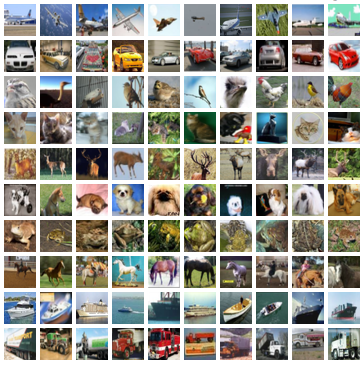
\includegraphics[width=0.5\textwidth]{cifar10}
\caption{10 случайных изображений из каждого класса}
\end{figure}

\subsection{Фреймворк Caffe}
Свёрточные нейронные сети обучались с помощью фреймворка для глубокого обучения Caffe \cite{jia2014caffe}.
Изначально Caffe разрабатывался командой BVLC (Berkeley Vision and Learning Center), но постепенно перерос в большой 
open-source проект.\footnote{\url{https://github.com/BVLC/caffe}} На данный момент вклад в развитие Caffe внесли почти 200 
разработчиков и более 10\,000 человек оценили проект на Github.

Данный фреймворк был выбран для решения задачи по нескольким причинам:
\begin{enumerate}
    \item Простота определения моделей и методов оптимизации. Архитектуры нейронных сетей
    (Caffe поддерживает топологии сетей в форме любых ациклических графов) и алгоритмы оптимизации удобно и 
    эффективно определяются в специальных конфигурационных файлах типа Google Protocol 
    Buffers\footnote{\url{https://developers.google.com/protocol-buffers/}}. 
    \item Модульность. Caffe позволяет легко изменять архитектуру сети под новые форматы входных данных. Кроме того, в наличии 
    имеется много слоёв и функций потерь.
    \item Скорость вычислений и эффективное использование ресурсов. Caffe заранее выделяет ровно столько памяти сколько нужно для 
    нейронной сети. Операций линейной алгебры такие как умножение, сложение и свёртка выполняются на CPU с помощью BLAS (Basic 
    Linear Algebra Subroutines). На GPU за эти операции отвечают библиотеки cuBLAS и cuDNN 
    \cite{DBLP:journals/corr/ChetlurWVCTCS14}
    \item CLI и интерфейсы для Python и Matlab.
\end{enumerate}

Caffe написан на языках C++, Cuda, Python. Для хранения датасетов используются эффективные базы данных 
LMDB\footnote{\url{http://symas.com/mdb/}} и LevelDB\footnote{\url{https://github.com/google/leveldb}}. Обучение нейронных сетей 
может выполняться как на CPU, так и на нескольких GPU одновременно. Фреймворк доступен для Linux, Windows и OS X.

\subsection{Предварительная обработка данных}
Необработанные изображения содержат излишнюю информацию, так как смежные пиксели имеют высокую корреляцию. Поэтому прежде чем 
подавать изображения на вход нейронной сети, они были обработаны в два этапа. В начале была произведена глобальная нормализация контраста
(global contrast normalization):
\[ \widehat{X} = \cfrac{X - \overline{X}}{\sigma},\]
где $X$ --- исходное изображение, $\overline{X}$ --- среднее значение, $\sigma$ --- стандартное отклонение.

Затем изображения были линейно трансформированы с помощью ZCA whitening \cite{learningmultiple}.
Цель данного алгоритма сделать входные изображения слабо коррелирующими друг с другом.

\begin{lstlisting}[language=Python, frame=TB, caption=Алгоритм ZCA whitening]
cov = np.dot(X.T, X) / X.shape[0] #%* Вычисляем ковариационную матрицу *)
U,S,V = np.linalg.svd(cov) #%* Находим сигнулярное разложение ковариацонной матрицы *)
Xrot = np.dot(X, U) #%* Поворачиваем входные данные *)
Xwhite = Xrot / np.sqrt(S + %*$\alpha$*)) #%* Делим на собственные числа *)
\end{lstlisting}
\vspace*{-0.4cm}
\begin{figure}[h]
    \centering
    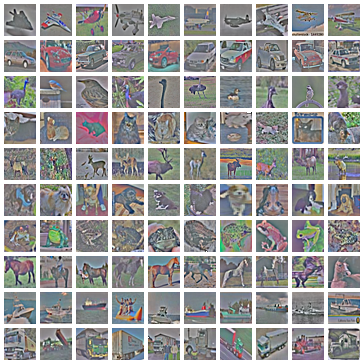
\includegraphics[width=0.5\textwidth]{cifar10zca}
    \caption{Изображения после применения ZCA whitening с параметром $\alpha=0,1$}
\end{figure}
Предобработка с помощью ZCA whitening уменьшила ошибку в среднем на $1,5\%$. Кроме того, каждое изображение было
увеличено до 40$\times$40 пикселей, для того чтобы в процессе обучения вырезать из 
изображения случайный патч размером 32$\times$32. Такой приём позволяет снизить эффект переобучения модели и повысить конечную 
точность распознавания.

\subsection{Обучение нейронных сетей}
Во время исследования были проверены различные гипотезы, архитектуры и эвристики так или иначе влияющие на конечные точности 
моделей. В результате различных экспериментов были отобраны семь нейронных сетей, показавшие наилучший результат.
В приложении отражены топологии сетей (таблица~\ref{models-table}), графики обучения (рисунок~\ref{fig:train_all}) и время,
затраченное на обучение каждой из моделей (рисунок~\ref{time_consumption}).

\subsubsection{Инициализация параметров}
Оптимизационные алгоритмы для глубоких нейронных сетей являются итеративными и, таким образом, требуют
от пользователя задания начальной точки, с которой нужно начать обучение. От выбора этой точки определятся
конечная сходимость алгоритма. Более того, выбор начальной точки определяет с какой скоростью
будет проходить обучение и какова будет ошибка в конечной точке, к которой сойдётся оптимизационный алгоритм.

Современные стратегии инициализации просты и основаны на различных эвристиках. Проектирование более сложных методов
является трудной задачей, так как оптимизация нейронных сетей ещё не достаточно изучена. В данной работе инициализация
проводилась с помощью layer-sequential unit-variance~\cite{DBLP:journals/corr/MishkinM15}.
Данный метод сначала проводит преинициализацию случайными ортонормированными матрицами~\cite{DBLP:journals/corr/SaxeMG13},
затем, последовательно для каждого слоя настраивает весовые коэффициенты таким образом, чтобы дисперсия
выходных данных слоя была единичной. Эксперименты показали, что такая инициализация позволяет эффективно 
обучать очень глубокие нейронные сети. Далее будут описаны отобранные для конечного ансамбля модели, их архитектуры, 
свойства и особенности обучения.

\subsubsection{Модель I}
Модель I состоит из 18 обучающихся слоёв и $\approx$\,2,7 млн. параметров.
Данная нейронная сеть достигла самой высокой точности предсказания среди всех обученных моделей (93,4\%). 
Maxout в качестве функции активации является её отличительной особенностью.
На рисунке~\ref{fig:model_I_maxout_example} показано как maxout соединён с выходами свёрточных слоёв. На
рисунке~\ref{fig:model_I_maxout_ip_example} можно видеть соединение выходов полносвязного слоя и активации.

\begin{figure}[H]
\centering
\begin{minipage}{.5\textwidth}
  \centering
  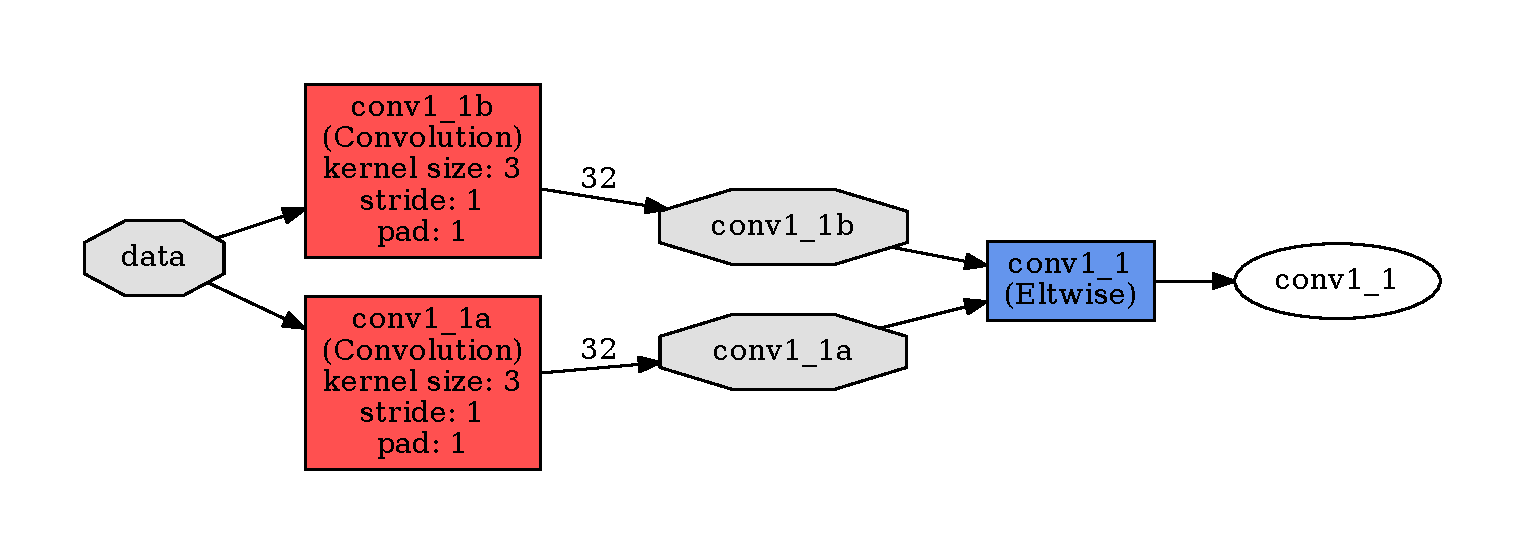
\includegraphics[width=\textwidth]{model_I_maxout_example}
  \captionof{figure}{Соединение maxout со\\
                     свёрточными слоями}
  \label{fig:model_I_maxout_example}
\end{minipage}%
\begin{minipage}{.5\textwidth}
  \centering
  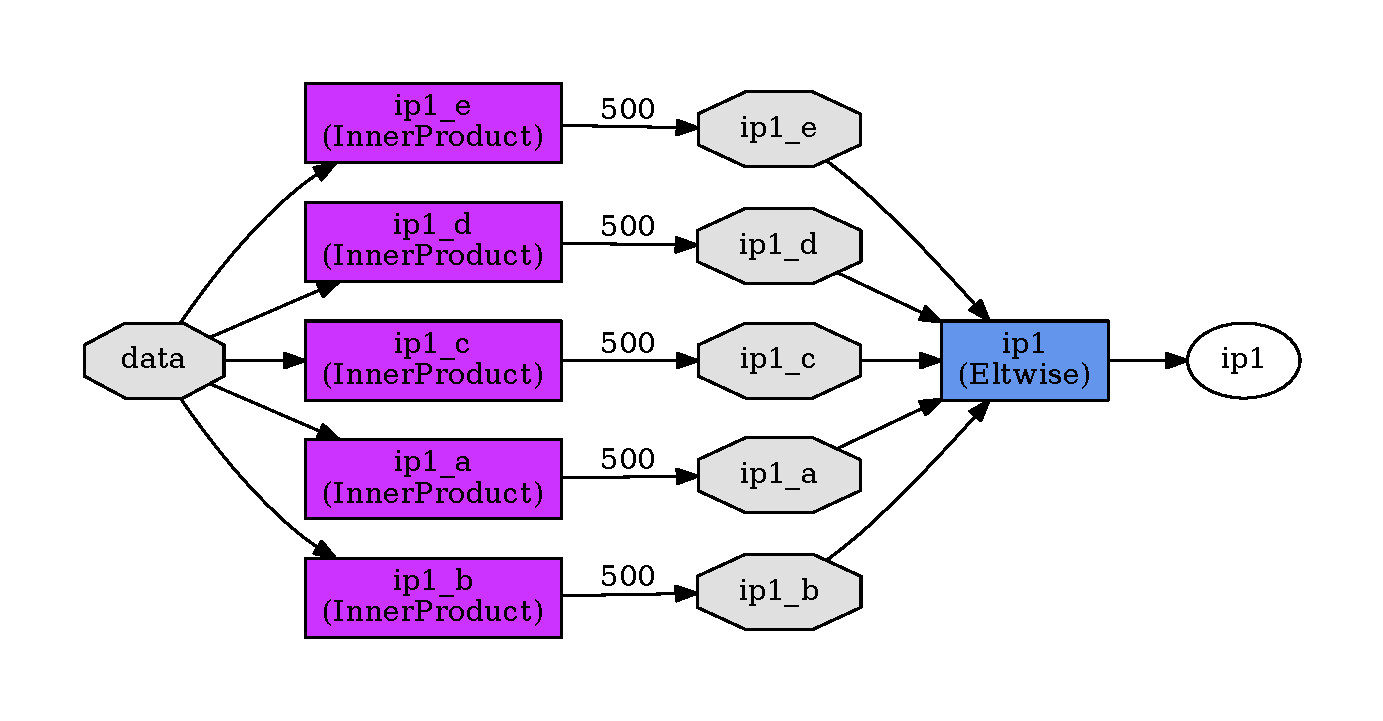
\includegraphics[width=\textwidth]{model_I_maxout_ip_example}
  \captionof{figure}{Соединение maxout с\\
                     полносвязными слоями}
  \label{fig:model_I_maxout_ip_example}
  \vspace*{1.4cm}
\end{minipage}
\vspace*{-1.4cm}
\end{figure}

Нейронная сеть обучалась 90\,000 итераций методом стохастического градиентного спуска,
с начальным learning rate (lr) 0,01, моментом 0.9, L2 регуляризацией с коэффициентом 0,0005 и 
мини батчем (mini batch) из 256 изображений. В процессе обучения, начиная с 40\,000 итерации, 
lr уменьшался в десять раз каждые 20\,000 итераций, достигнув к концу обучения значения $10^{-5}$.

\begin{figure}[H]
    \centering
    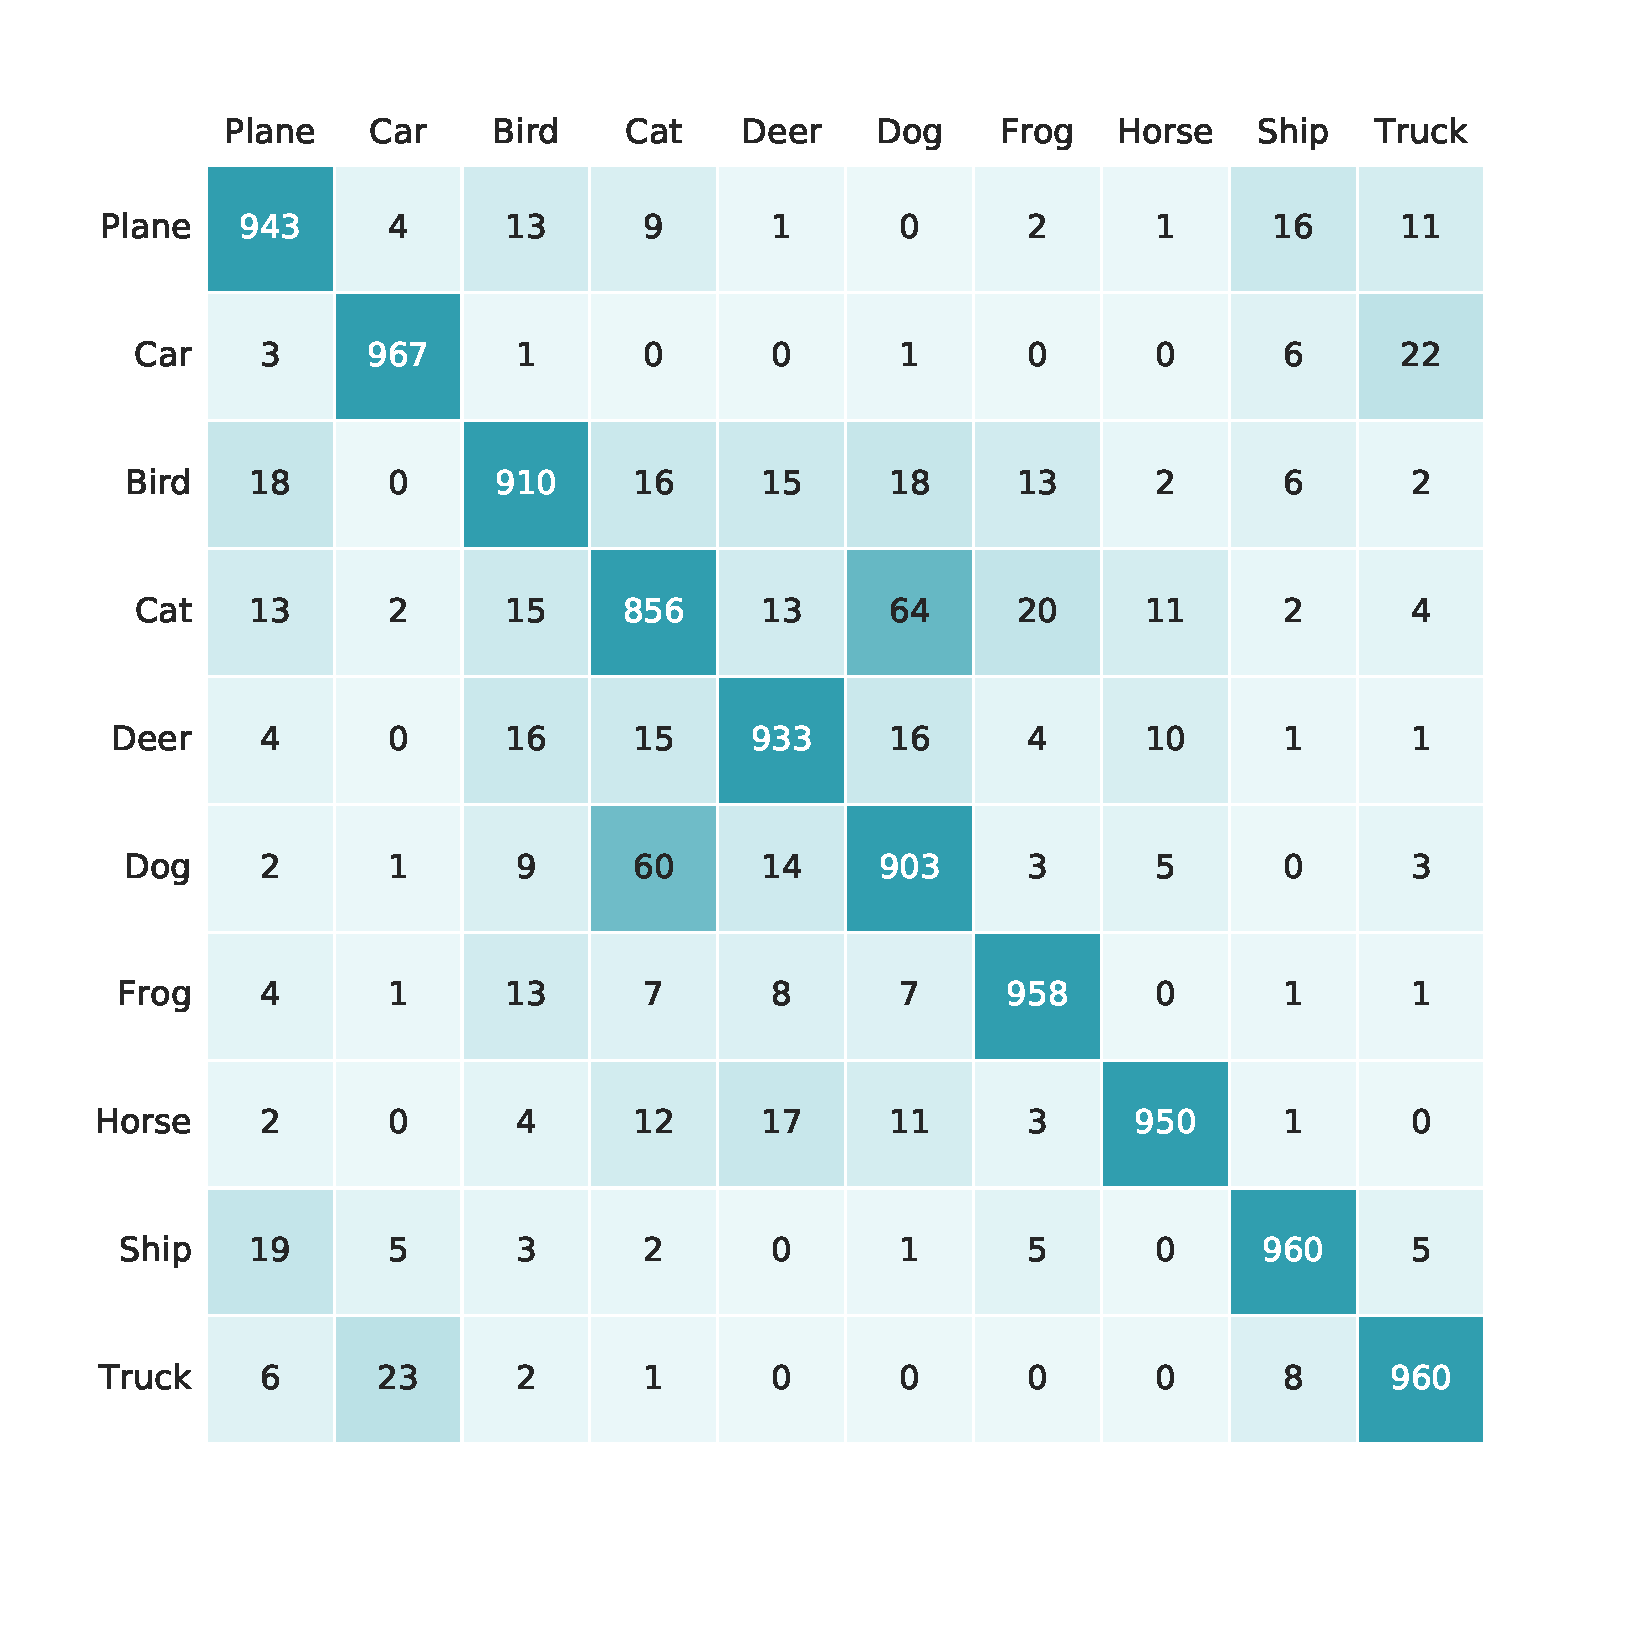
\includegraphics[width=0.6\textwidth]{confusion_matrix_model_I}
    \vspace*{-1cm}
    \caption{Матрица предсказаний модели I}
    \label{fig:confusion_matrix_model_I}
\end{figure}

\subsubsection{Модели II и III}
Модель II имеет в 4,5 раза меньше параметров, в сравнении с моделью I ($\approx$\,600\,000).
Данная нейронная сеть имеет классическую архитектуру --- чередование свёрточных и pooling слоёв, в качестве
функции активации используется Leaky ReLU\footnote{$f(x) = \max(x, \alpha x)$} с параметром $\alpha = 0,01$.

Сеть обучалась в течении 30\,000 итераций. Функционал ошибки оптимизировался алгоритмом NAG (Nesterov accelerated gradient)
\cite{SutskeverMartensDahlHinton_icml2013}, с начальным learning rate (lr) 0,01, моментом 0.9, L2 регуляризацией с коэффициентом 0,0005 и 
мини батчем из 256 изображений. Начиная с 15\,000 итерации, 
lr уменьшался в десять раз каждые 5\,000 итераций, достигнув к концу обучения значения $10^{-5}$.

Результат модели II оказался ниже на тестовом множестве, в сравнении с моделью I (89,48\% против 93,4\%).
Данный результат объясняется недообучением, что является следствием недостаточного числа параметров в нейронной сети.
С другой стороны, за счёт уменьшения числа весов в модели, удалось снизить время обучения в 10 раз (с десяти часов до одного).

Модель III является попыткой исправить главный недостаток модели II за счёт увеличения числа параметров.
В связи с чем, число фильтров каждого свёрточного слоя было увеличено в два раза, что позволило снизить ошибку на 1,55\%.
Параметры оптимизации использовались такие же как в модели II.

\begin{figure}[H]
\centering
\begin{minipage}{.5\textwidth}
  \centering
  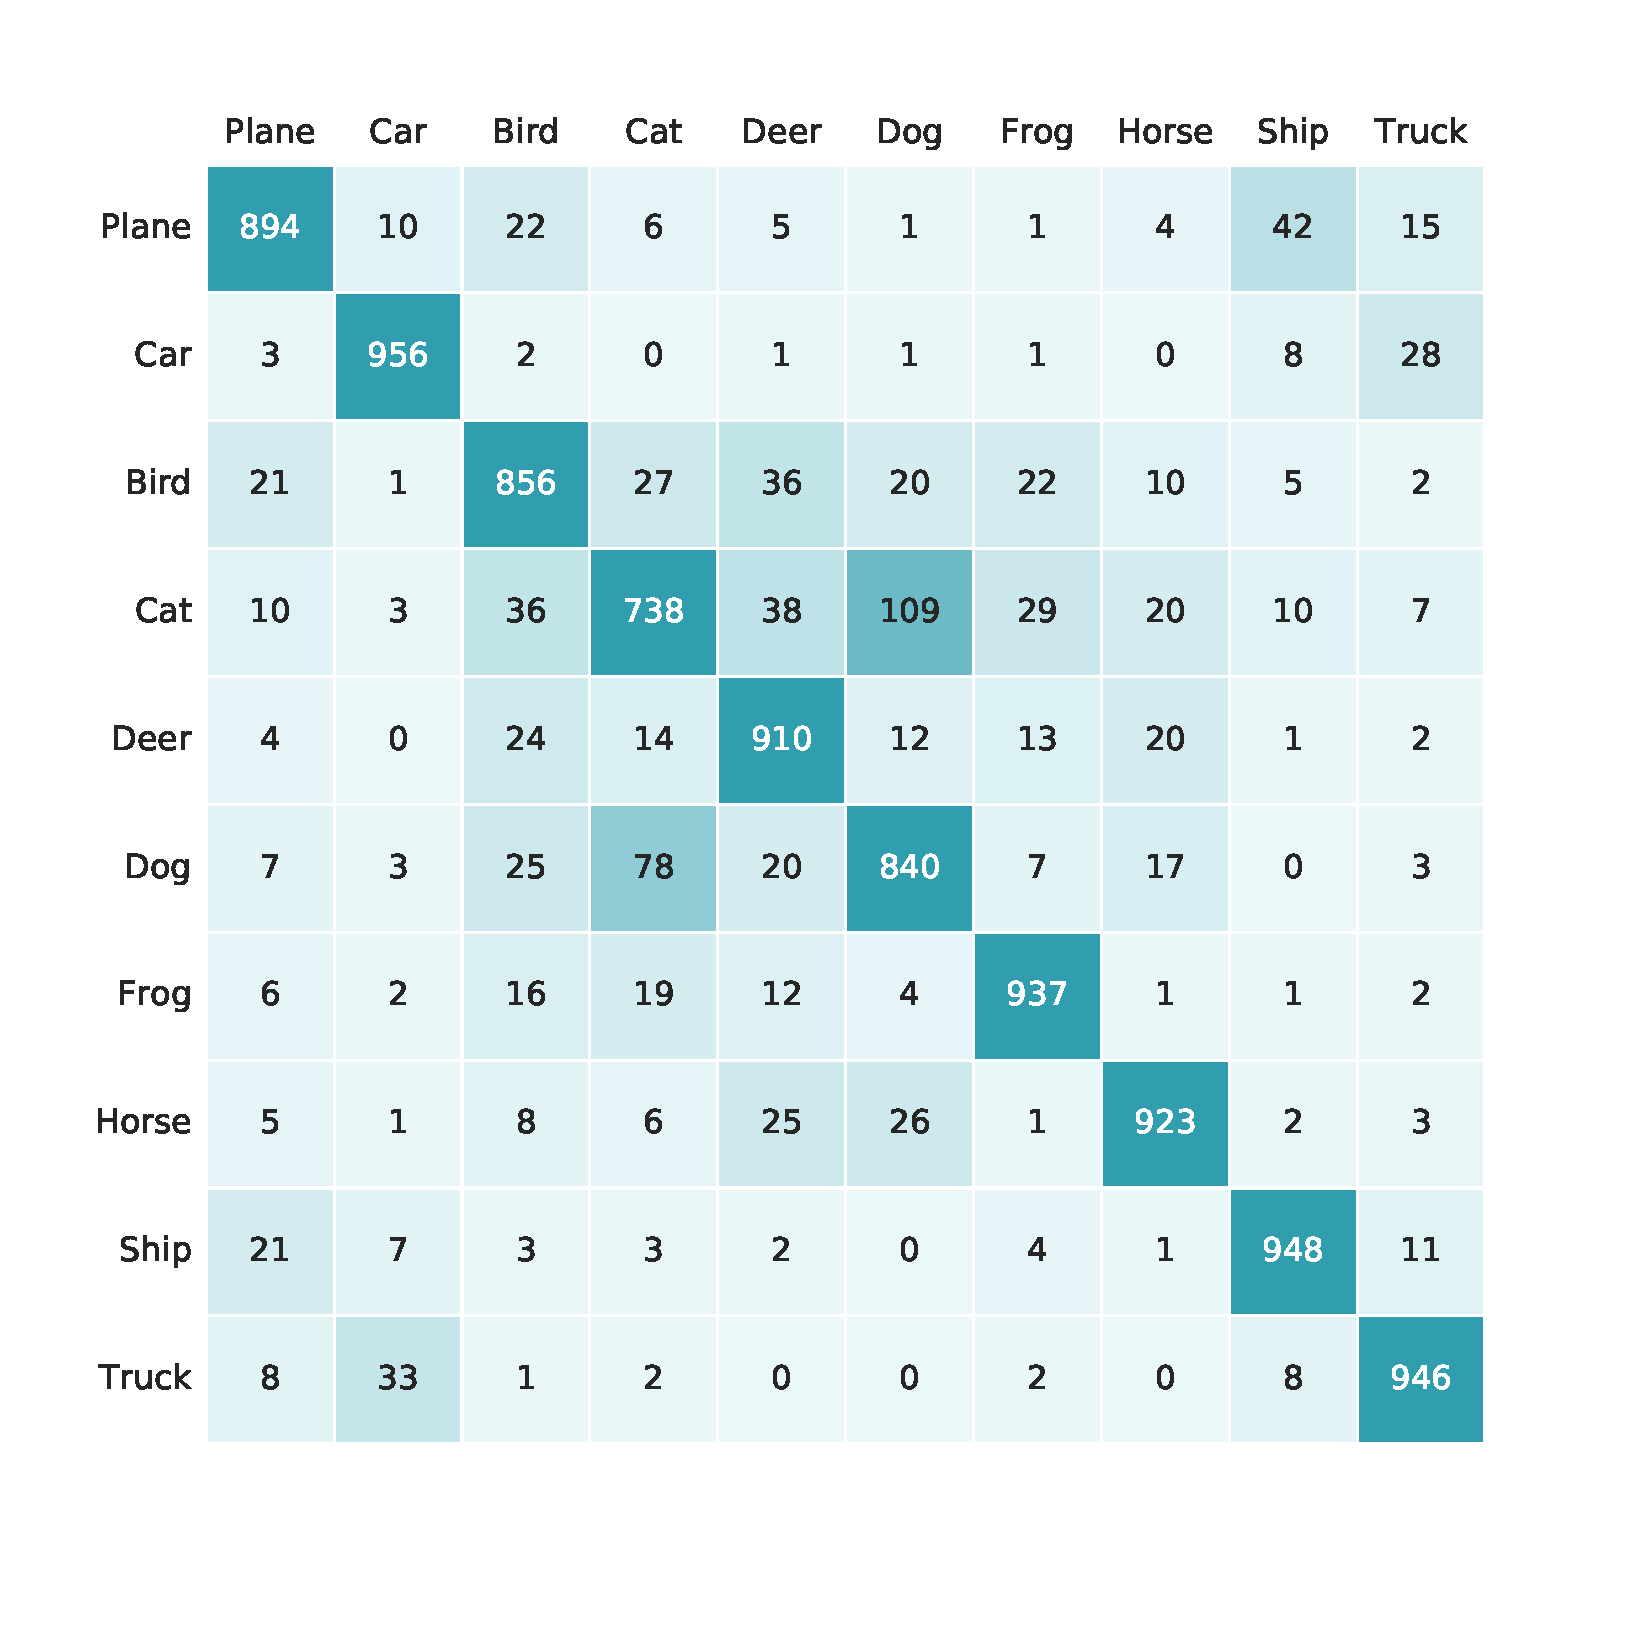
\includegraphics[width=\textwidth]{confusion_matrix_model_II}
  \vspace*{-1.7cm}
  \captionof{figure}{Матрица предсказаний\\модели II}
\end{minipage}%
\begin{minipage}{.5\textwidth}
  \centering
  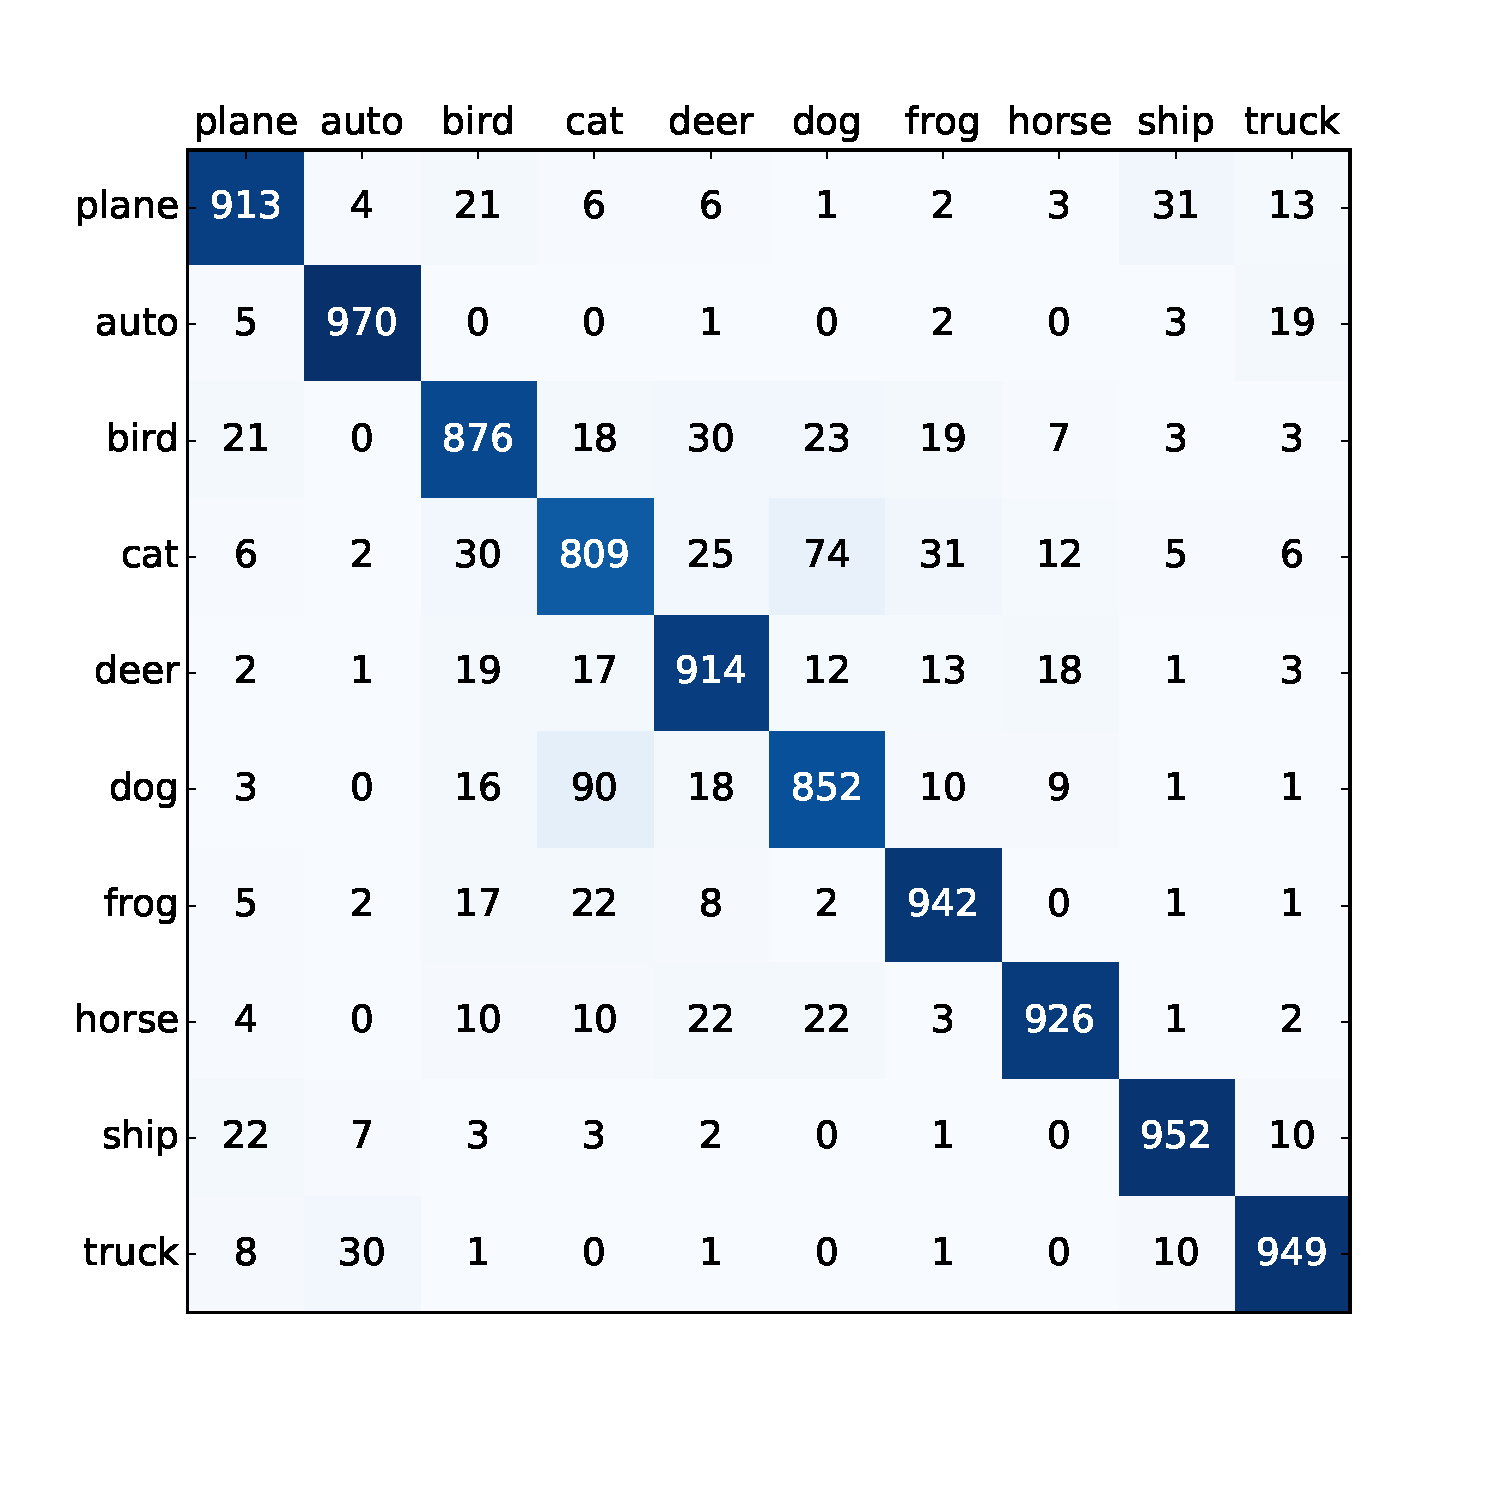
\includegraphics[width=\textwidth]{confusion_matrix_model_III}
  \vspace*{-1.7cm}
  \captionof{figure}{Матрица предсказаний\\модели III}
\end{minipage}
\end{figure}

\subsubsection{Модели IV и V}
На моделях IV и V проверялась гипотеза, что pooling слои могут быть заменены на соответствующие свёрточные слои
с увеличенным параметром stride без значительного снижения точности распознавания. \cite{DBLP:journals/corr/SpringenbergDBR14}.
В данных сетях max-pooling~2$\times$2 слои были заменены  на свёрточные слои со stride равным двум.

Модель IV имеет $\approx$\,6 млн. параметров и 13 слоёв. В качестве функции активации используется ReLU.
Параметры оптимизации использовались такие же как и в моделях II и III, за исключением увеличенного
до 50\,0000 числа итераций SGD. После обучения в течении 14 часов, точность на тестовом множестве достигла 92,1\%, что
подтверждает гипотезу о замене pooling слоёв.

Модель V состоит из 16 слоёв и $\approx$\,7,8 млн свободных параметров. Данная нейронная сеть является попыткой
улучшить точность модели IV за счёт увеличения числа свёрточных слоёв. Однако, дополнительные слои привнесли
дополнительно $\approx$\,1,8 млн. параметров, что привело к переобучению и снижении конечной точности на 1,19\%.
Модель V обучалась в течении 19 часов, с мини батчем из 128 изображений и используя такие же оптимизационные параметры
как и модель IV.

\begin{figure}[H]
\centering
\begin{minipage}{.5\textwidth}
  \centering
  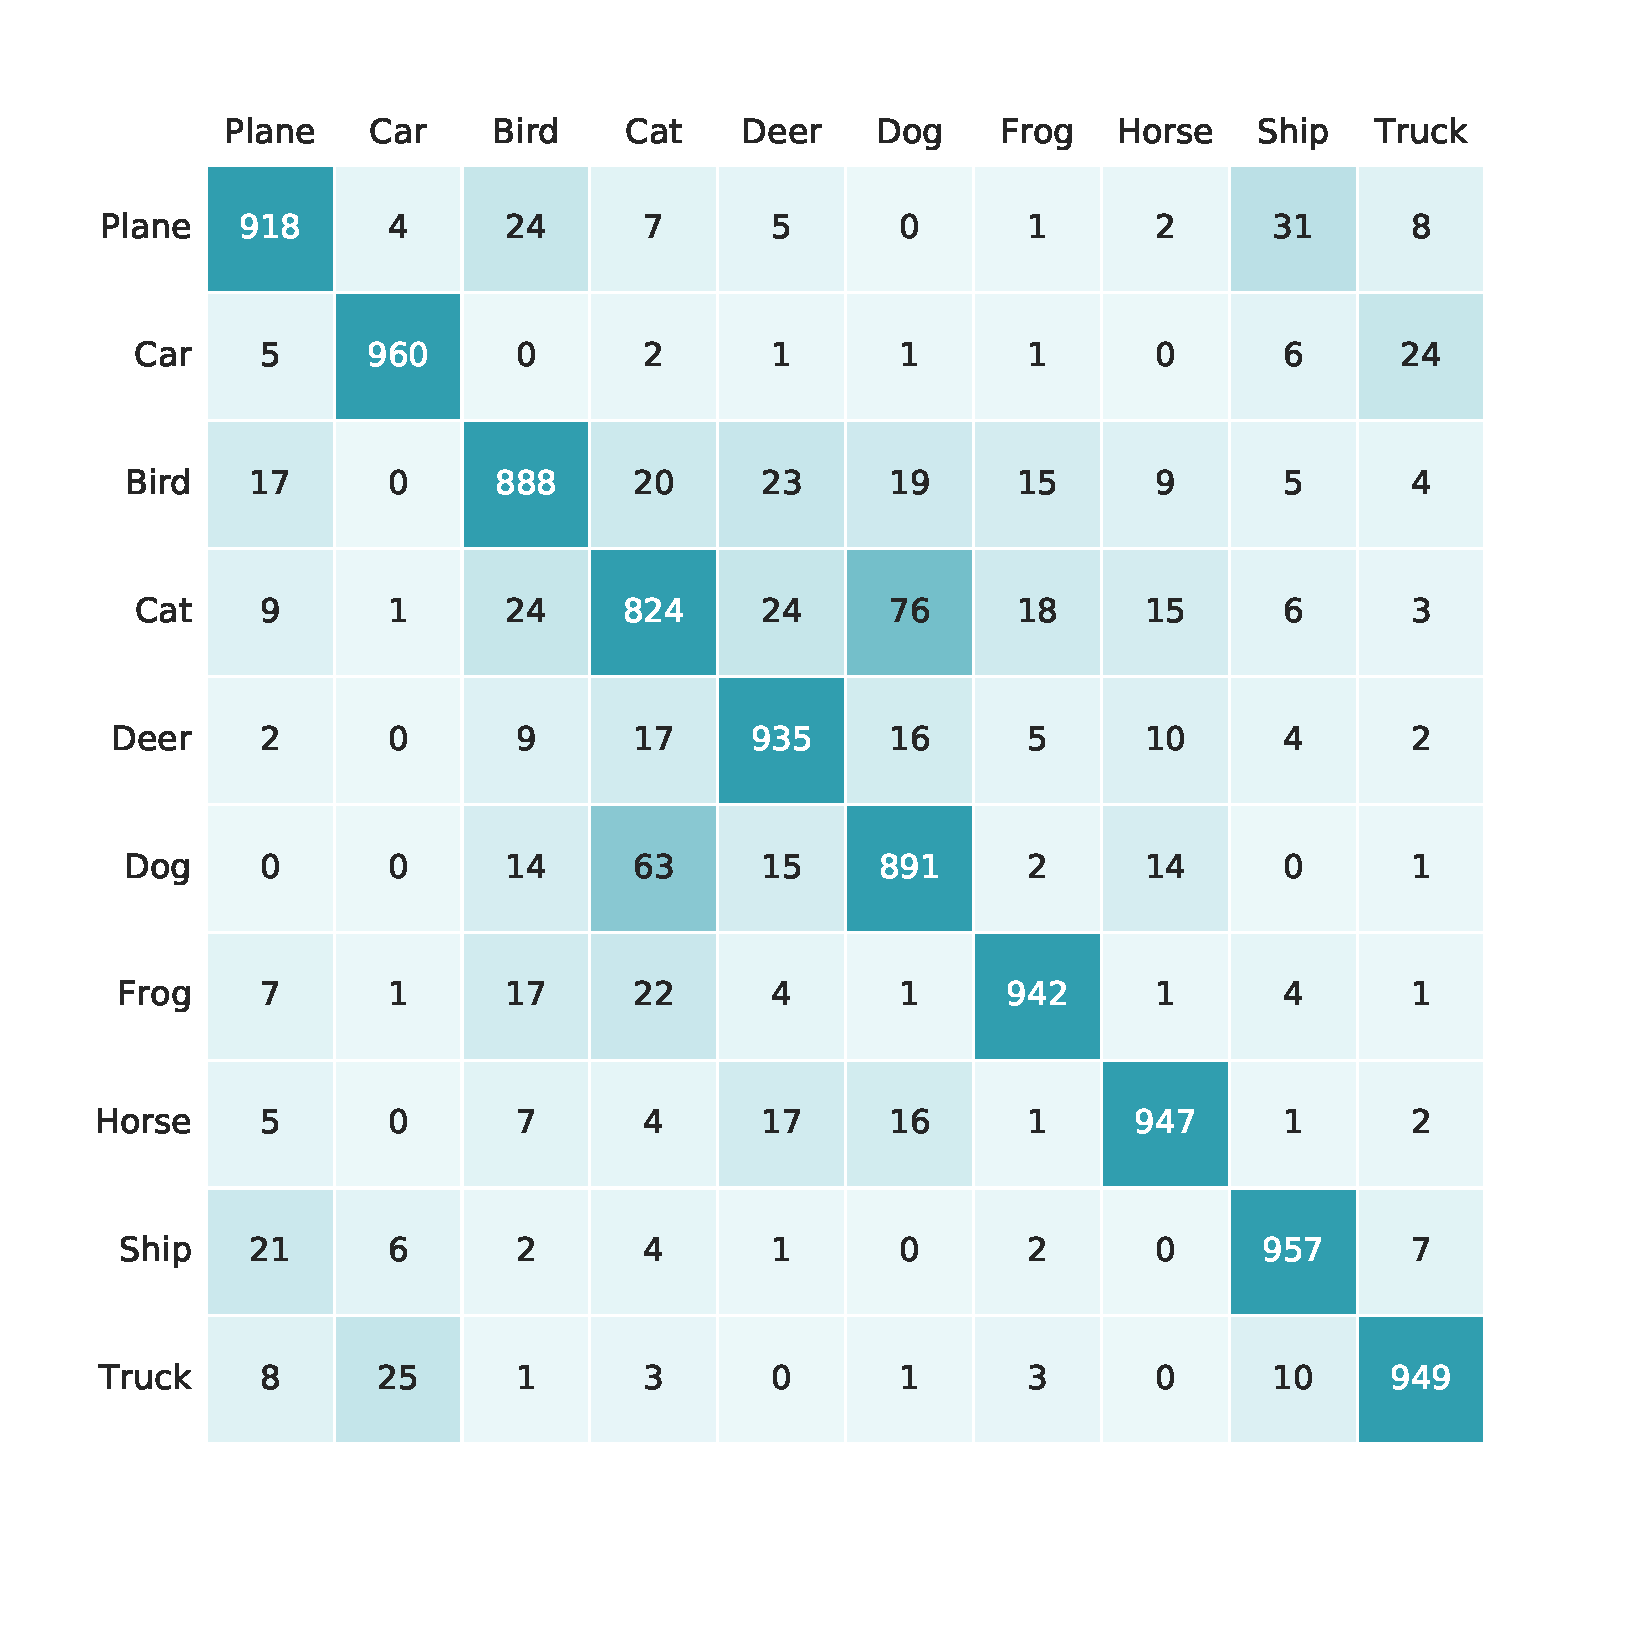
\includegraphics[width=\textwidth]{confusion_matrix_model_IV}
  \vspace*{-1.7cm}
  \captionof{figure}{Матрица предсказаний\\модели IV}
\end{minipage}%
\begin{minipage}{.5\textwidth}
  \centering
  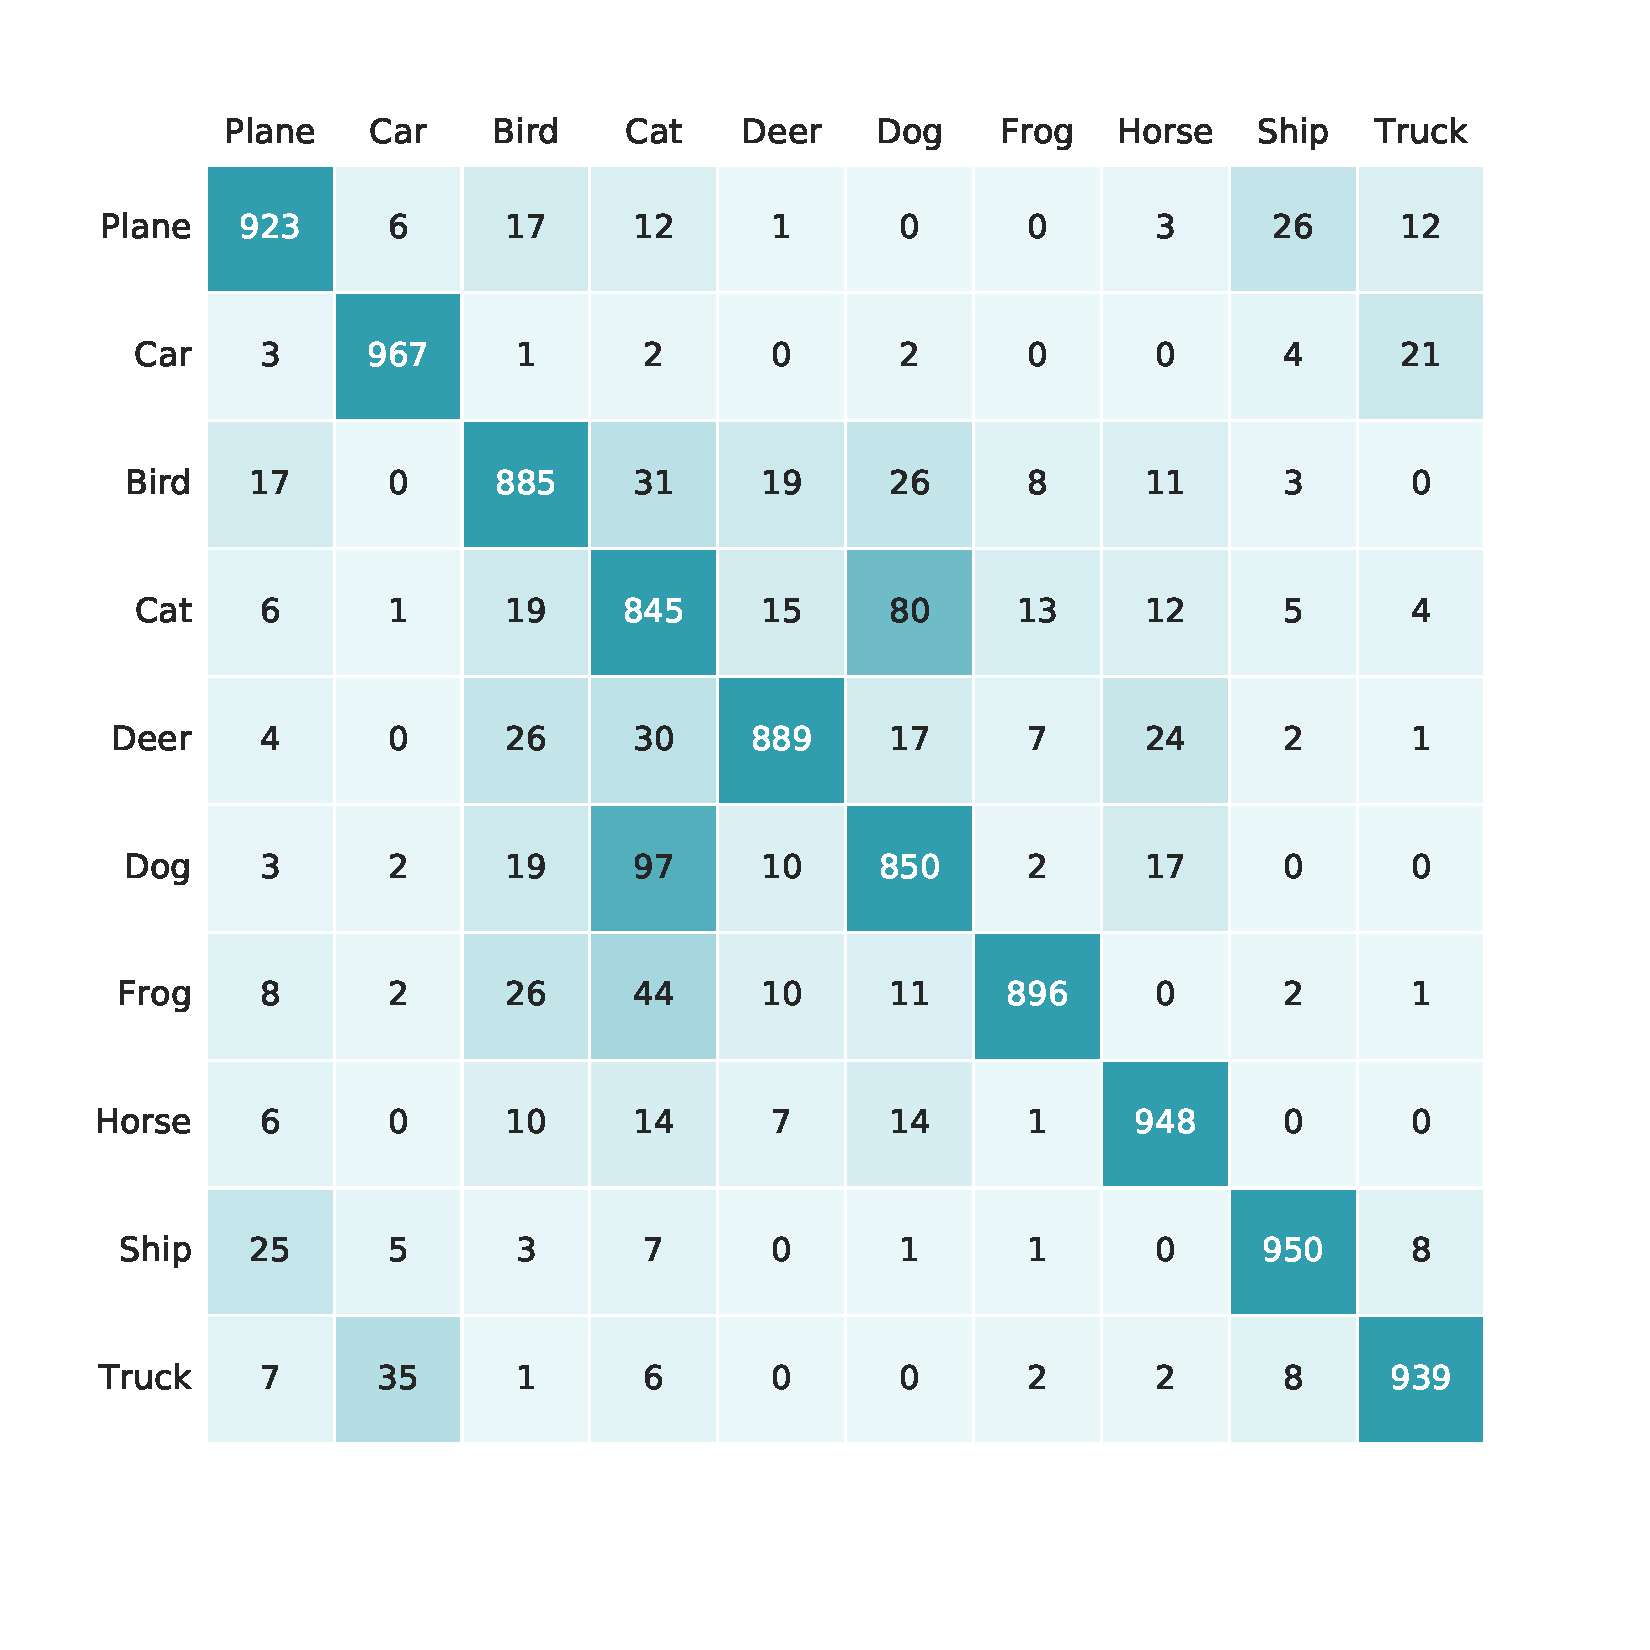
\includegraphics[width=\textwidth]{confusion_matrix_model_V}
  \vspace*{-1.7cm}
  \captionof{figure}{Матрица предсказаний\\модели V}
\end{minipage}
\end{figure}

\subsubsection{Модель VI}
Модель VI состоит из 18 слоёв и $\approx$\,4,2 млн. параметров. Данная модель использует слои batch normalization, 
которые преобразовывают активации свёрточных и полносвязных слоев таким образом, что их среднее равно нулю, а
дисперсия единице (значения вычисляются на всём mini batch). Авторы batch normalization \cite{DBLP:journals/corr/IoffeS15}
утверждают, что данный приём позволяет использовать высокий learning rate и приводит к более быстрой сходимости.
Данная нейронная сеть обучалась 70\,000 итераций с помощью SGD. Модель VI достигла точности в 92,0\% за 25\,0000 итераций, 
обучение сети заняло 10 часов.
\begin{figure}[H]
    \centering
    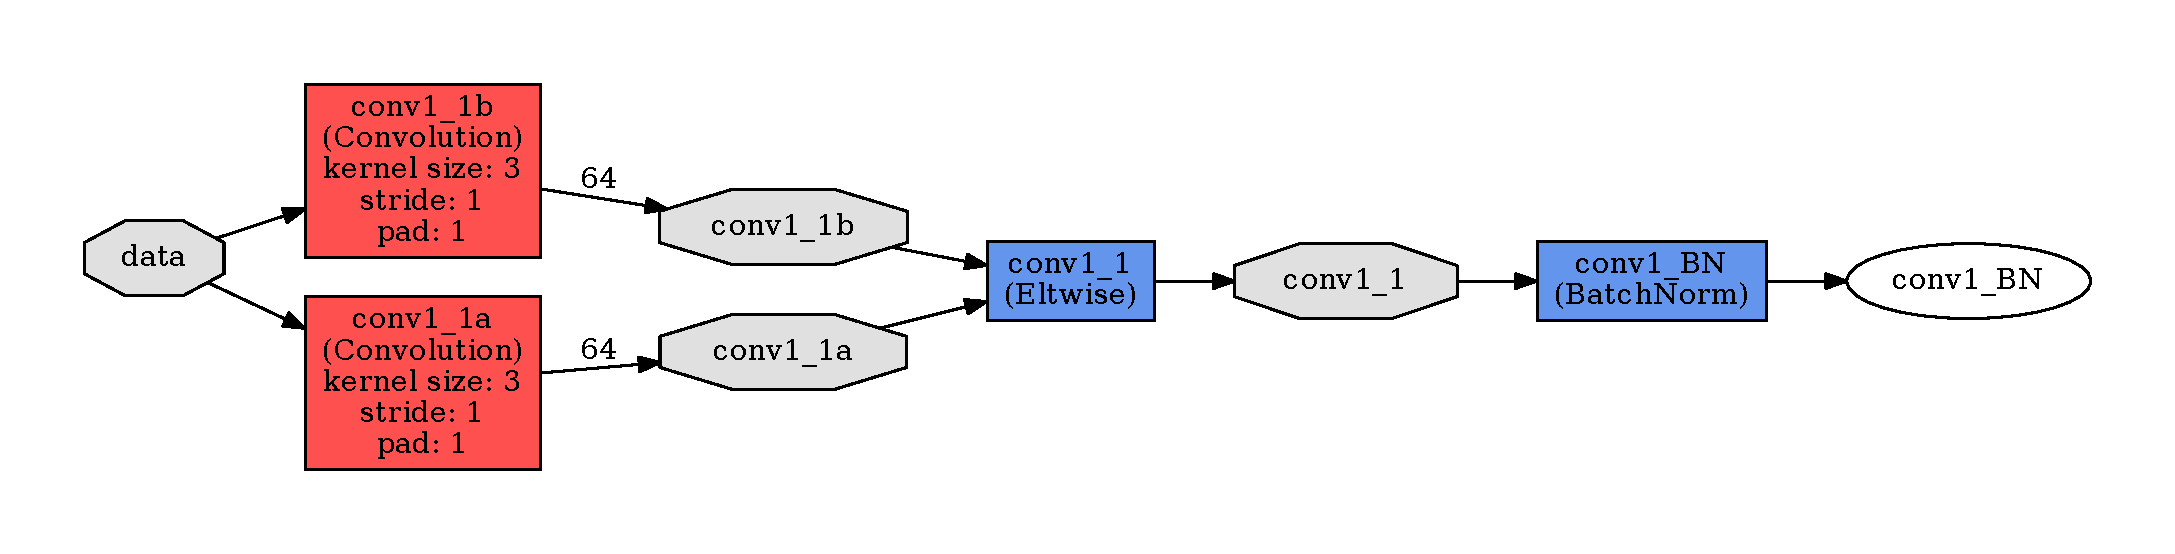
\includegraphics[width=0.9\textwidth]{batchnrm_net_VI}
    \caption{Batch normalization слой в модели~VI}
    \label{fig:model_VI_bnrm}
\end{figure}

\begin{figure}[H]
    \centering
    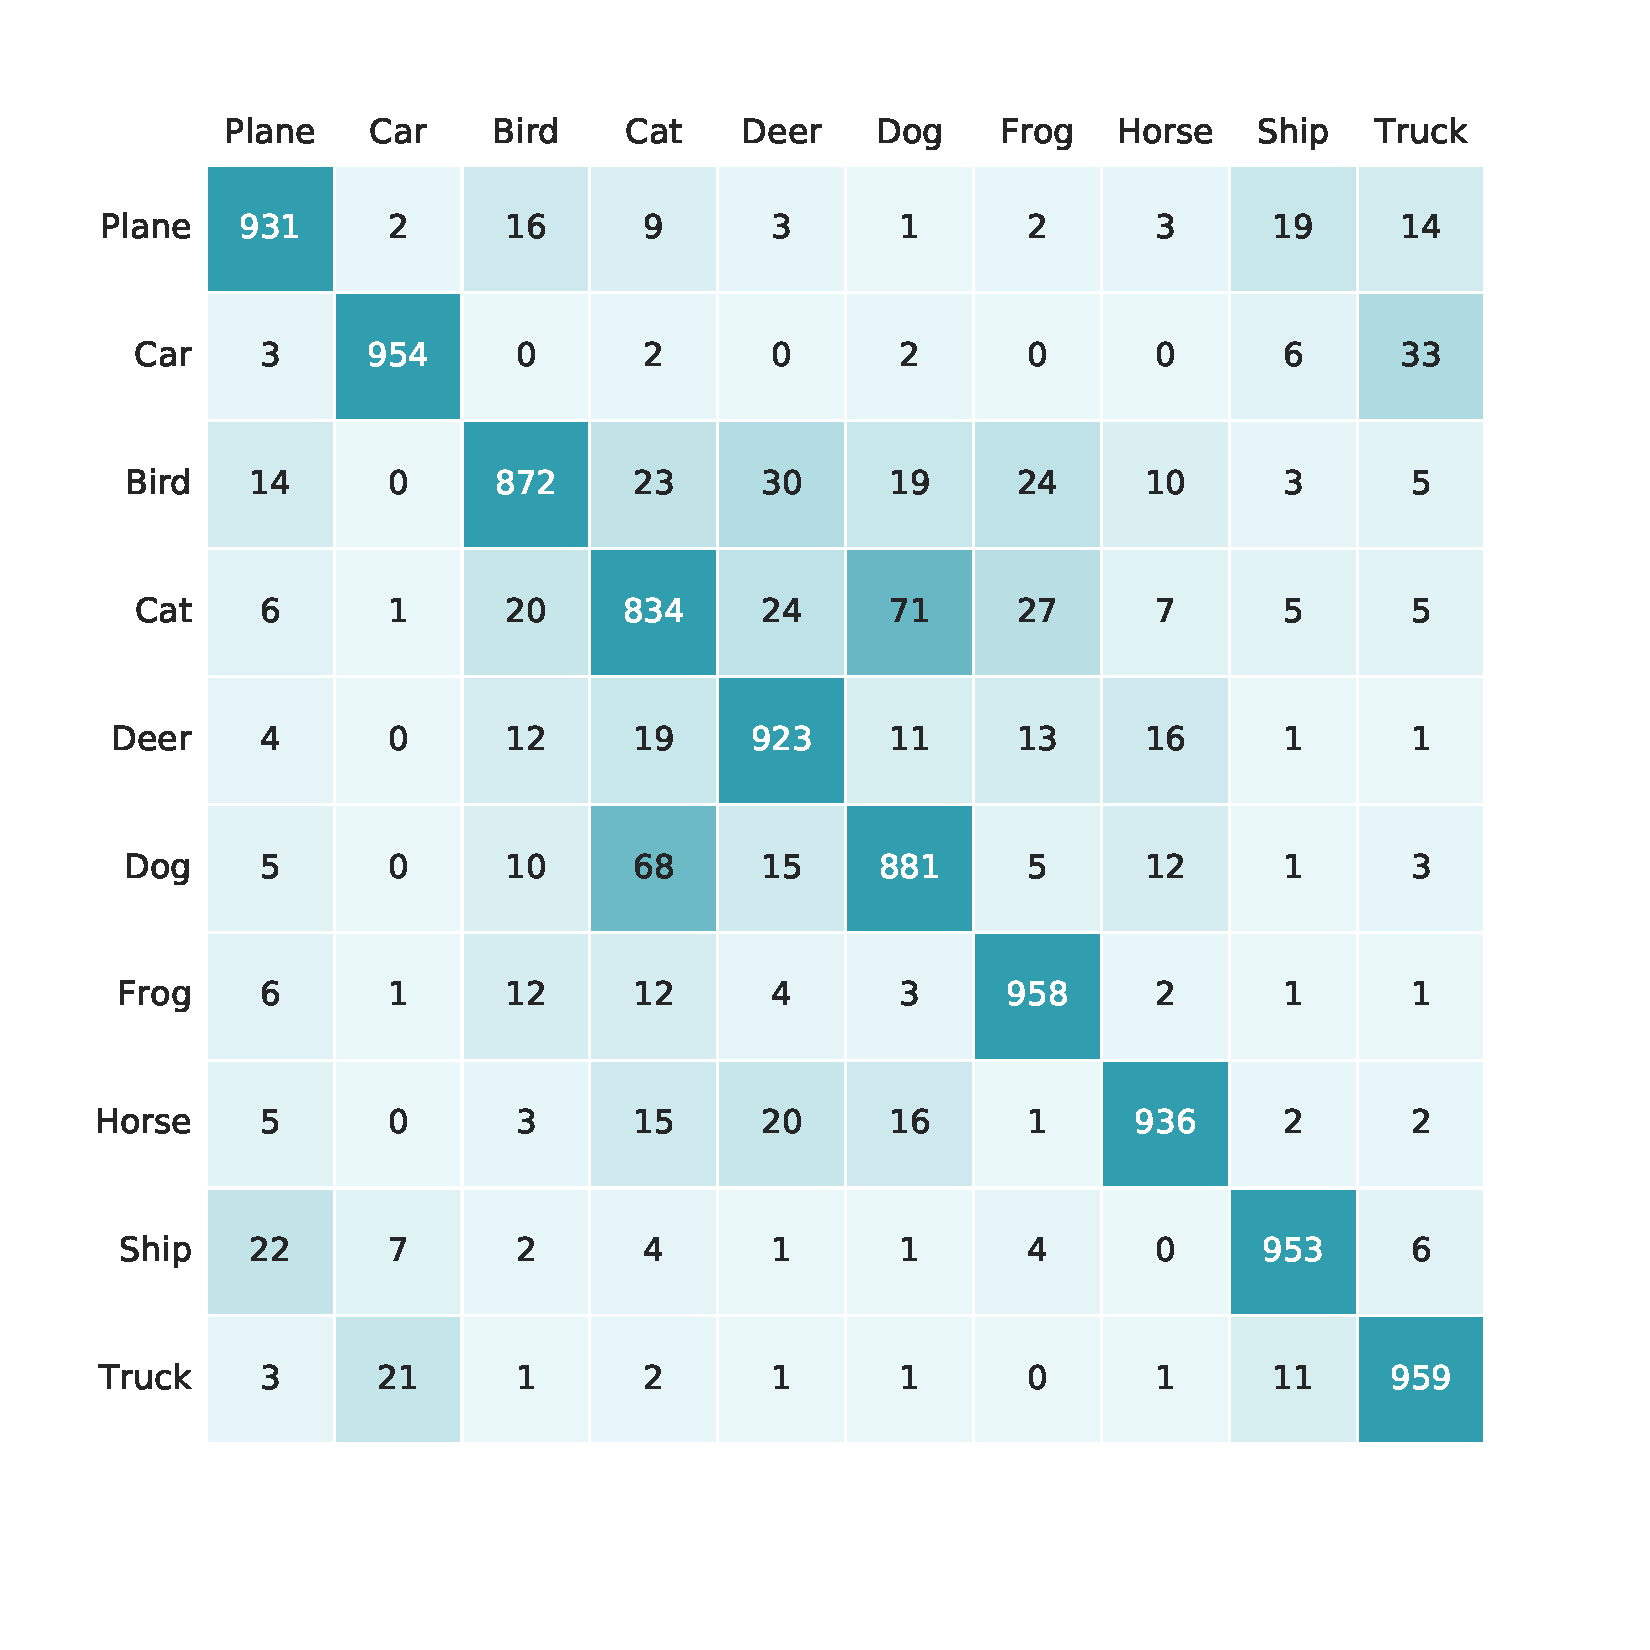
\includegraphics[width=0.5\textwidth]{confusion_matrix_model_VI}
    \vspace*{-1cm}
    \caption{Матрица предсказаний модели VI}
    \label{fig:confusion_matrix_model_VI}
\end{figure}

\subsubsection{Модель VII}
Модель VII идентична модели I, за исключением количества свёрточных слоёв соединённых с maxout активацией. В данной модели их пять
(Рис. \ref{fig:model_VII_maxout}), тогда как модель I имеет только два слоя. Такое изменение в топологии сети не привело к 
увеличению конечной точности модели, более того, ошибка увеличилась на 0,9\%. Максимальное число итераций достигло 70\,000,
время затраченное на обучение составило 22 часа.

\begin{figure}[H]
\centering
\begin{minipage}{.5\textwidth}
  \centering
  \vspace*{0.7cm}
  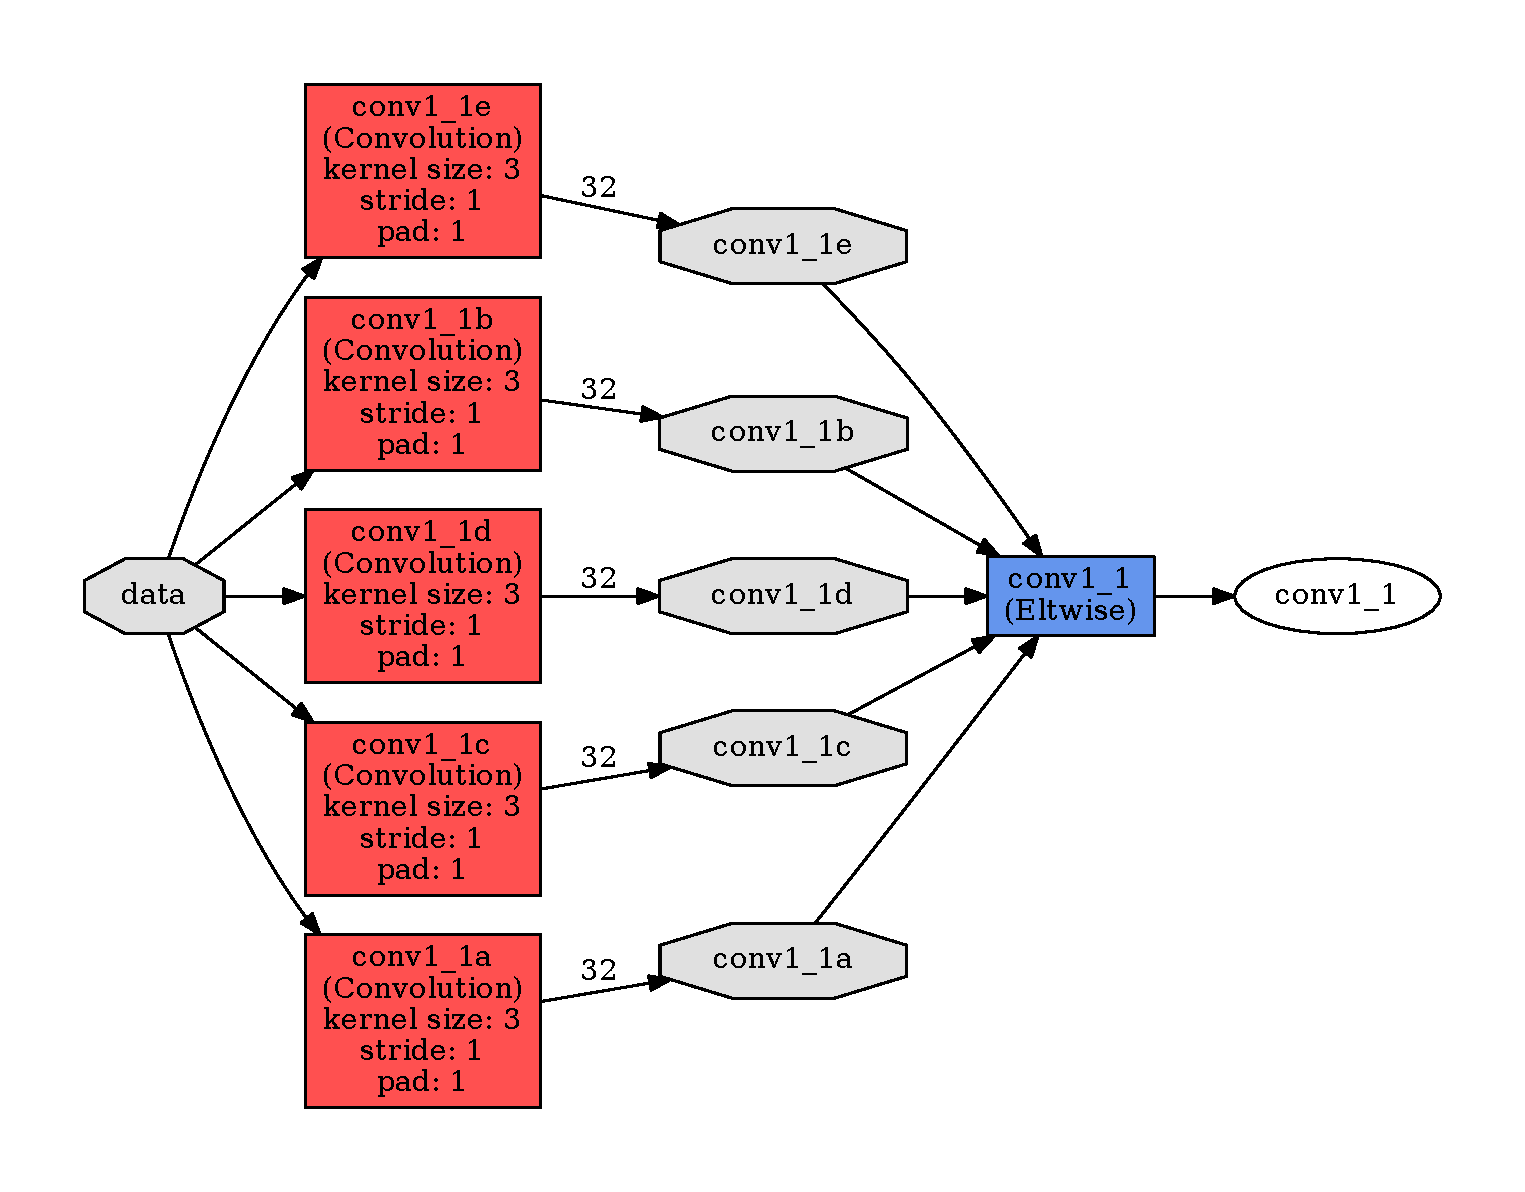
\includegraphics[width=\textwidth]{model_VII_maxout}
  \vspace*{-0.4cm}
  \captionof{figure}{Соединение maxout \\активаций в модели~VII}
  \label{fig:model_VII_maxout}
\end{minipage}%
\begin{minipage}{.5\textwidth}
  \centering
  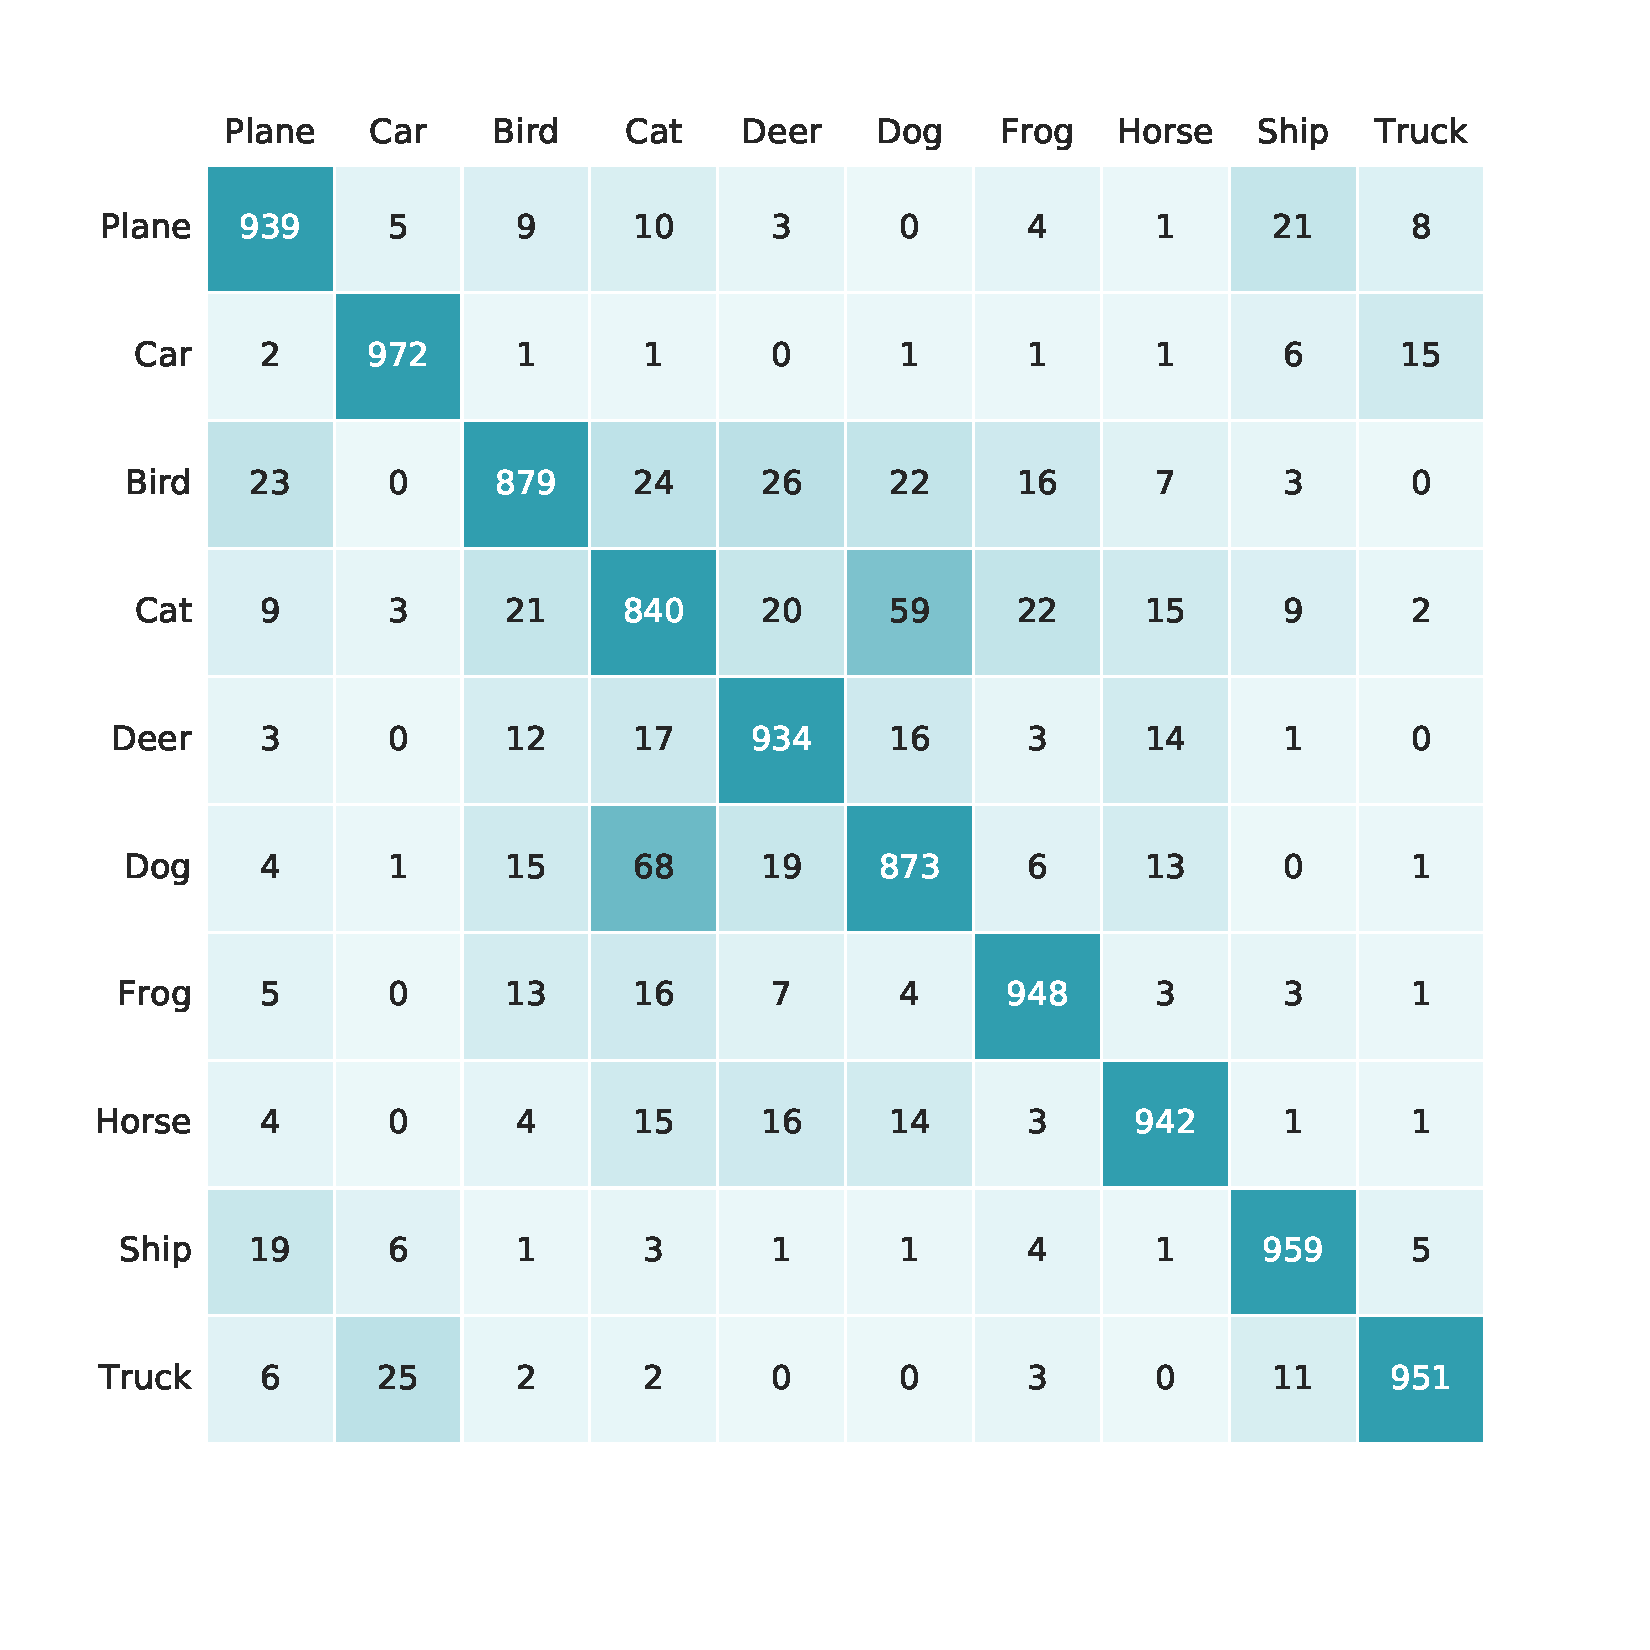
\includegraphics[width=\textwidth]{confusion_matrix_model_VII}
  \vspace*{-1.7cm}
  \captionof{figure}{Матрица предсказаний\\модели VII}
  \label{fig:confusion_matrix_model_VII}
\end{minipage}
\end{figure}

\subsection{Объединение нейронных сетей в ансамбль}
Объединение нескольких моделей в ансамбль является мощным приёмом при решении различных задач машинного обучения.
Применение подобной техники было выбрано по причине наличия различных свёрточных нейронных сетей, предсказания которых
не очень сильно коррелируют между собой. В данном исследовании создание ансамбля производилось при помощи <<стэкинга>> (stacking)
\cite{Wolpert92stackedgeneralization}, идея которого заключается в построении алгоритма, объединяющего
предсказания базовых моделей (в данном случае нейронных сетей). Такой подход зачастую работает лучше, 
так как усиливает обобщающую способность и робастность конечного классификатора за счёт одиночных моделей.

Для построения конечного ансамбля были протестированы различные алгоритмы классификации, такие как случайный лес,
метод k ближайших соседей, машина опорных векторов и Extra Trees. Наилучшая точность была достигнута с 
помощью алгоритма Extra Trees,\cite{ExtraTrees} (94,21\%), который сам является ансамблем 
деревьев решений. Схема объединения моделей отражена на рисунке \ref{fig:ansamble}.

\begin{figure}[H]
    \centering
    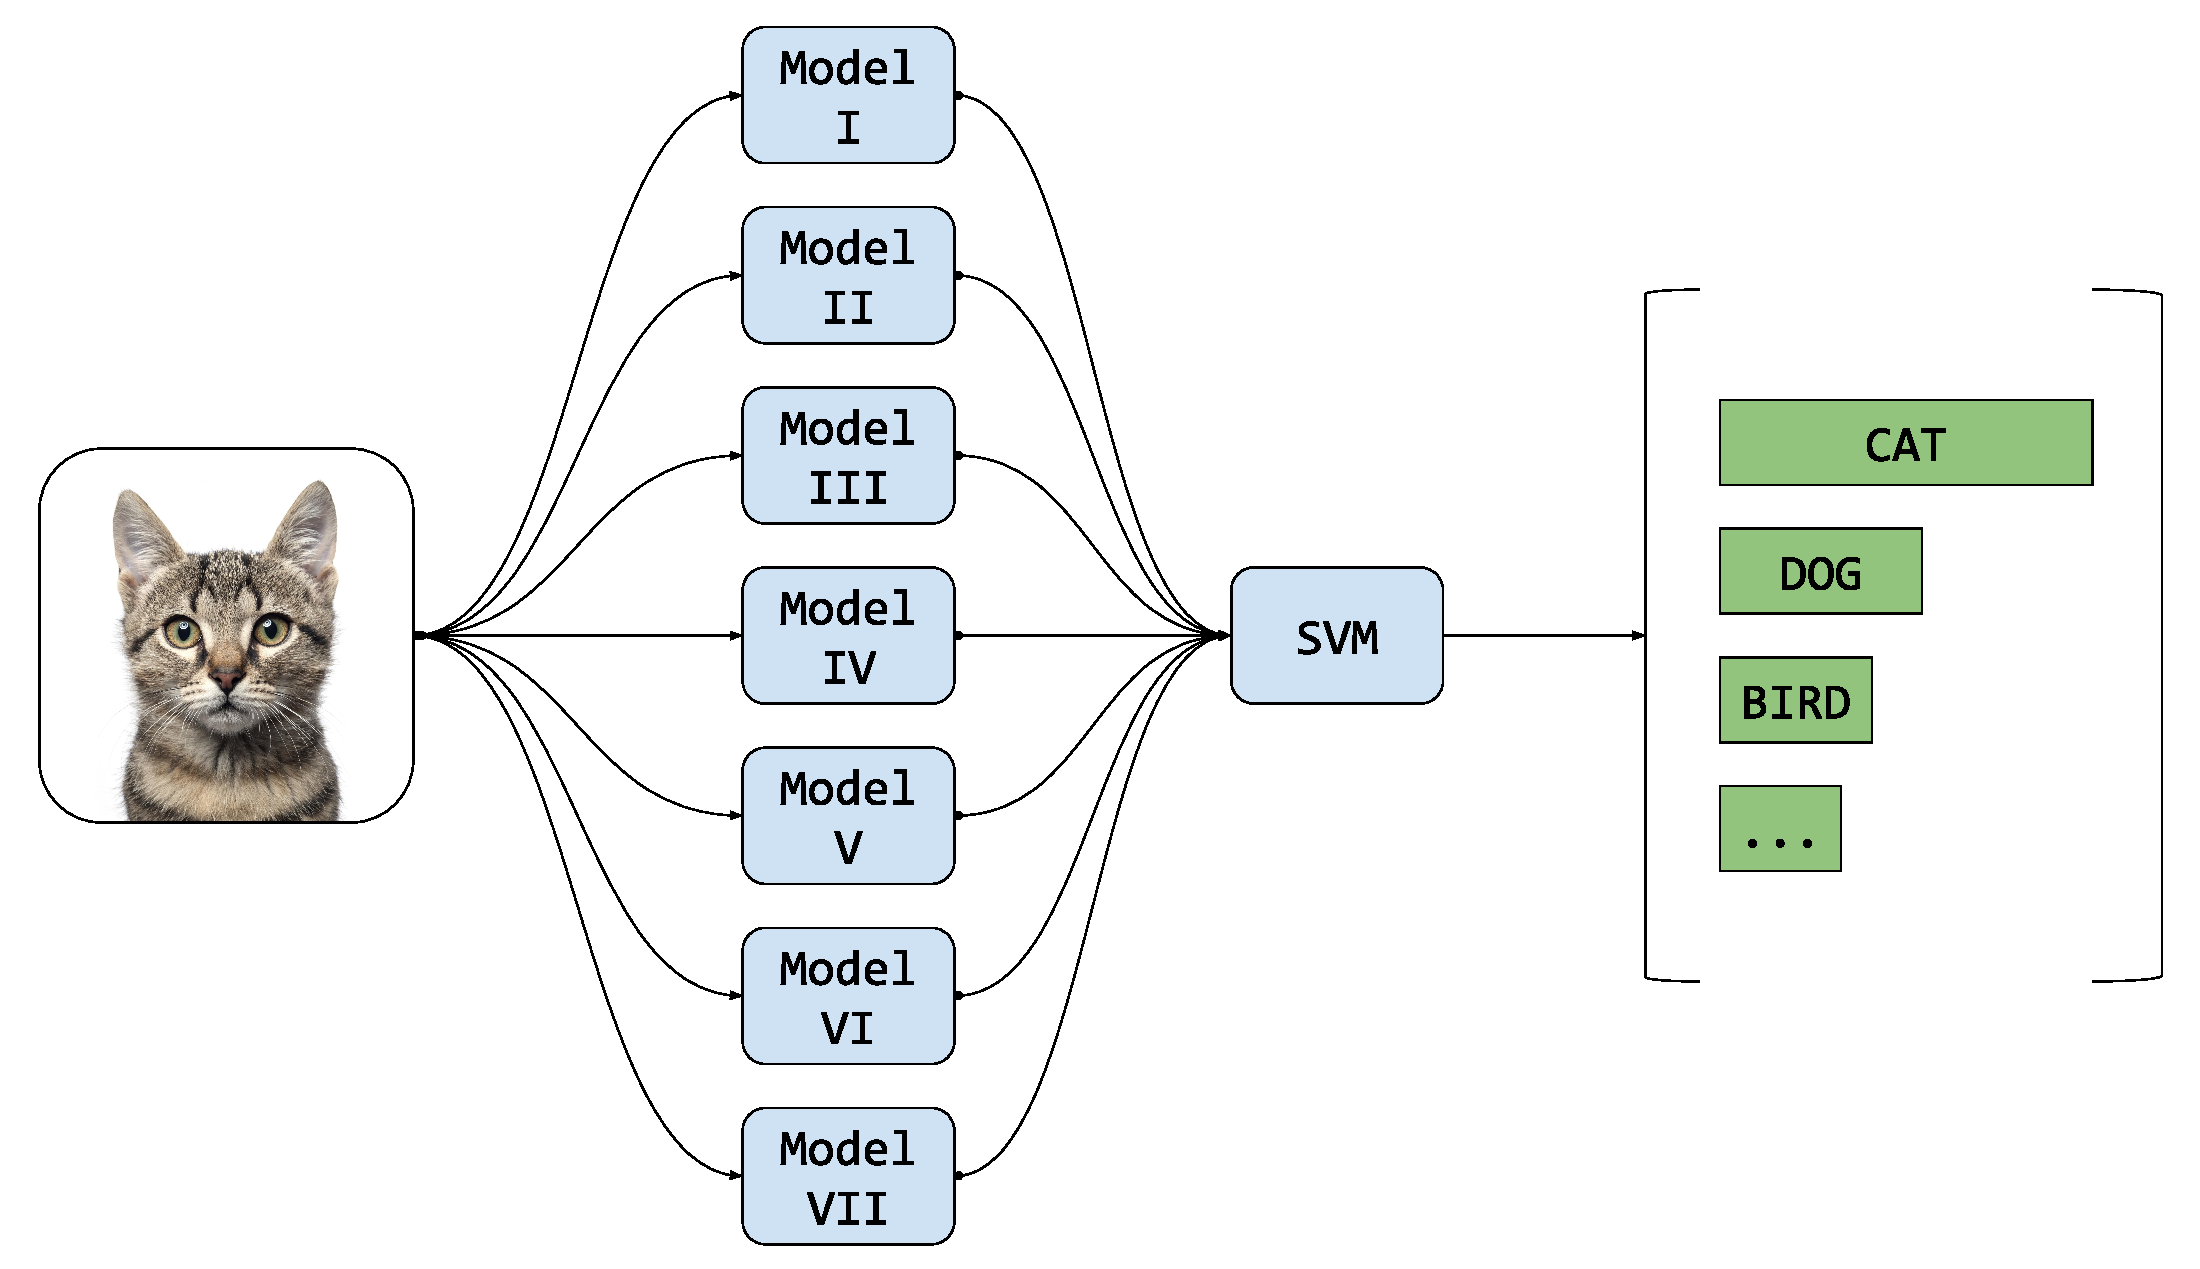
\includegraphics[width=0.9\textwidth]{ensamble}
    \caption{Схема конечного ансамбля}
    \label{fig:ansamble}
\end{figure}

\begin{figure}[H]
    \centering
    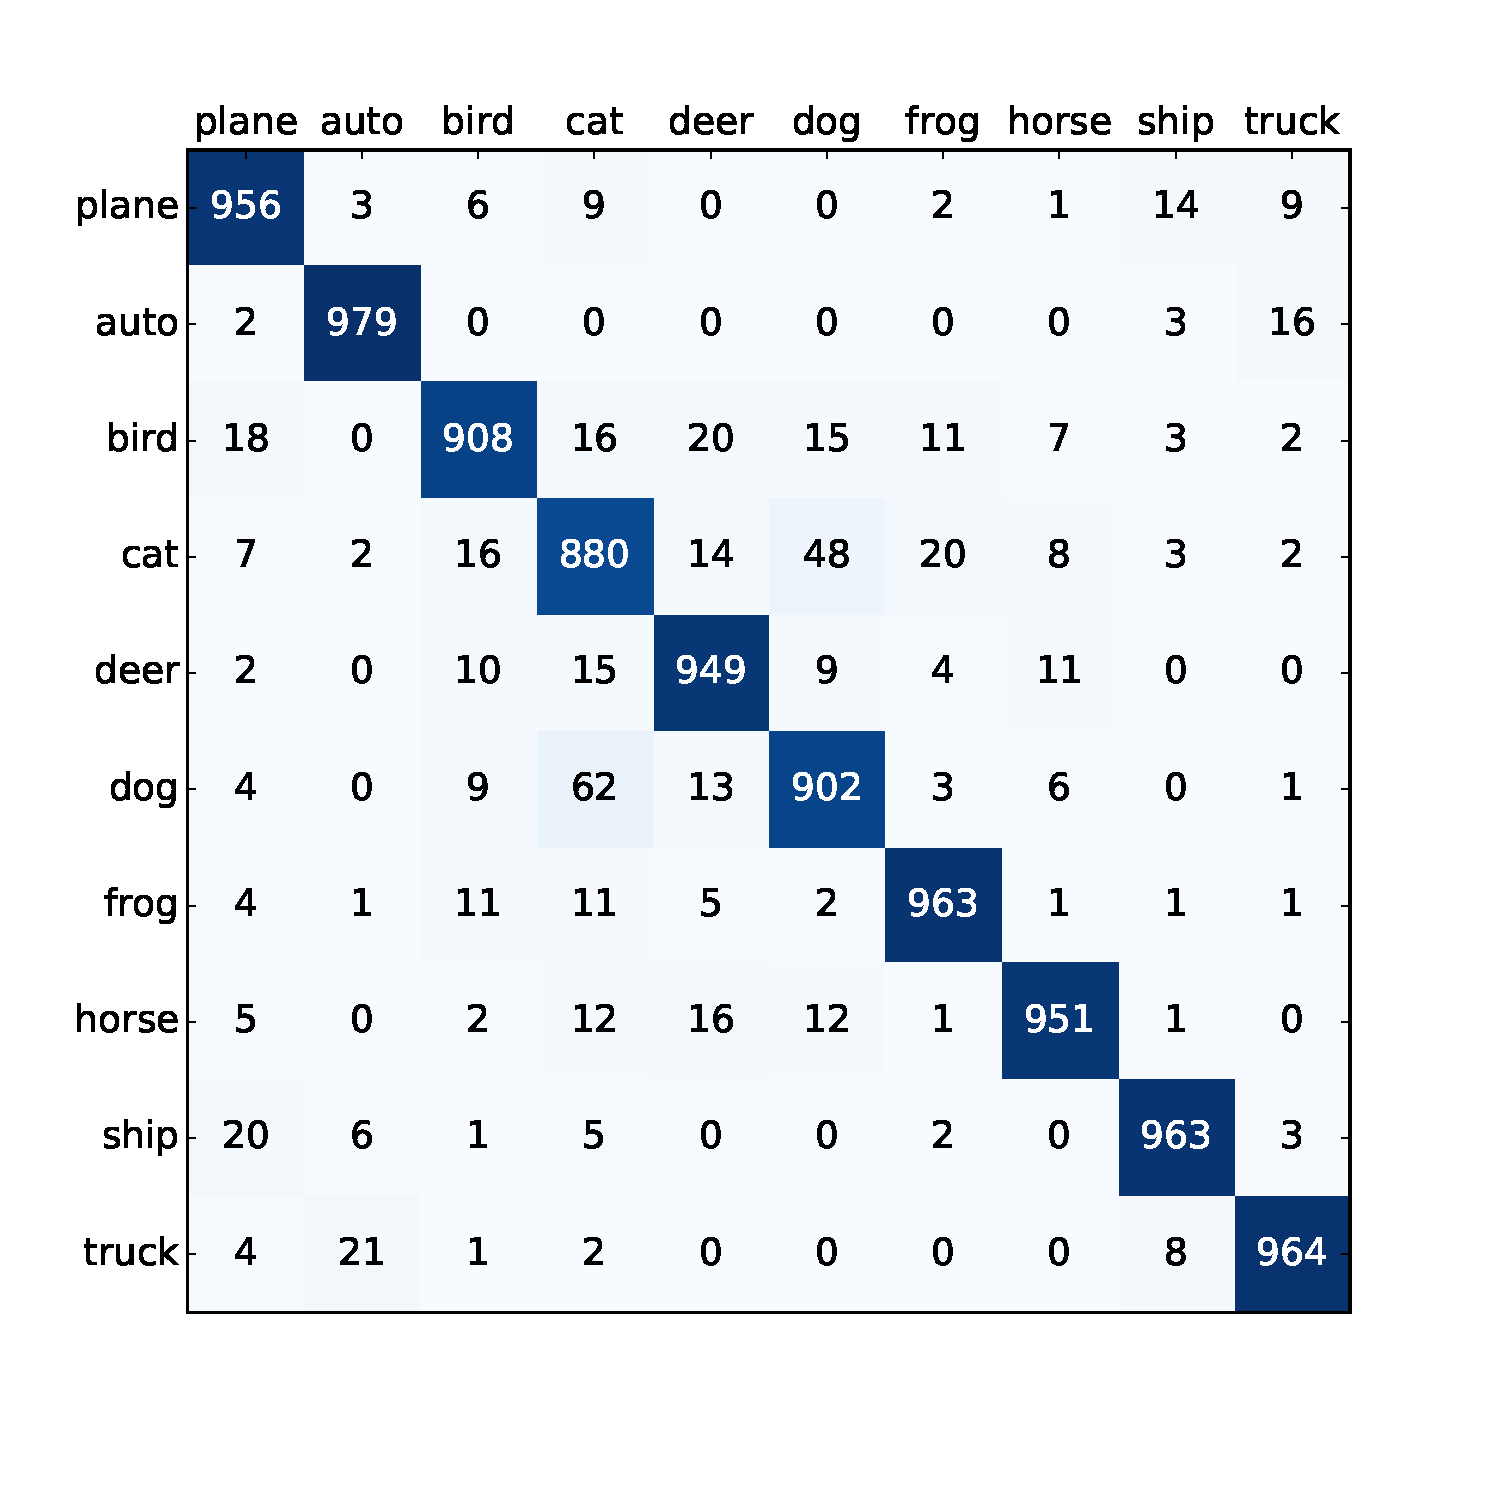
\includegraphics[width=0.7\textwidth]{ensamble_confusion_matrix}
    \vspace*{-1.3cm}
    \caption{Матрица предсказаний ансамбля моделей}
    \label{fig:ensamble_confusion_matrix}
\end{figure} % Основная часть
\section{Заключение}
В результате выполнения курсовой работы был спроектирован и обучен ансамбль моделей,
состоящий из семи различных глубоких свёрточных нейронных сетей и решающий задачу распознавания
образов на датасете CIFAR-10 с точностью, превосходящей точность распознавания человека.

В процессе исследования были получены теоретические знания в области машинного обучения,
анализа данных и глубокого обучения. В частности, были подробно изучены свёрточные нейронные 
сети, способы их проектирования, настройки и оптимизации, а также фреймворк Caffe, позволяющий
реализовывать модели и современные алгоритмы компьютерного зрения. Полученные знания послужат 
фундаментом для дальнейших исследований в этой области. Таким образом, по результатам работы можно 
сказать, что все поставленные задачи выполнены, цели достигнуты.


 % Заключение
\bibliography{biblio}
 % Список литературы
\setcounter{secnumdepth}{0}
\section{Приложение}
\begin{table}[h]
\resizebox{18cm}{!}{%
    \begin{tabular}{ccccccc}
    \toprule
    Model I          & Model II          & Model III          & Model IV                                                            & Model V                                                             & Model VI         & Model VII \\ \midrule
    conv1\_1 3x3x32  & conv1\_1 3x3x32   & conv1\_1 3x3x64    & conv1\_1 3x3x96                                                     & conv1\_1 3x3x96                                                     & conv1\_1 3x3x64   & conv1\_1 3x3x32    \\
    conv1\_2 3x3x32  & conv1\_2 3x3x32   & conv1\_2 3x3x64    & conv1\_2 3x3x96                                                     & conv1\_2 3x3x96                                                     & conv1\_2 3x3x64   & conv1\_2 3x3x32    \\
    conv1\_3 3x3x32  & conv1\_3 3x3x32   & conv1\_3 3x3x64    & conv1\_3 3x3x96                                                     & conv1\_3 3x3x96                                                     & conv1\_3 3x3x64   & conv1\_3 3x3x32    \\
    conv1\_4 3x3x48  & pool 2x2          & pool 2x2           & \begin{tabular}[c]{@{}c@{}}conv1\_4 3x3x96\\ stride 2\end{tabular}  & conv1\_4 3x3x96                                                     & conv1\_4 3x3x64   & conv1\_4 3x3x48    \\ 
    conv1\_5 3x3x48  & conv2\_1 3x3x64   & conv2\_1 3x3x128   & conv2\_1 3x3x192                                                    & \begin{tabular}[c]{@{}c@{}}conv1\_5 3x3x96\\ stride 2\end{tabular}  & conv1\_5 3x3x64   & conv1\_5 3x3x48    \\ 
    pool 2x2         & conv2\_2 3x3x64   & conv2\_2 3x3x128   & conv2\_2 3x3x192                                                    & conv2\_1 3x3x192                                                    & pool 2x2          & pool 2x2           \\   
    conv2\_1 3x3x80  & conv2\_3 3x3x64   & conv2\_3 3x3x128   & conv2\_3 3x3x192                                                    & conv2\_2 3x3x192                                                    & conv2\_1 3x3x128  & conv2\_1 3x3x80    \\
    conv2\_2 3x3x80  & conv2\_4 3x3x64   & conv2\_4 3x3x128   & \begin{tabular}[c]{@{}c@{}}conv2\_4 3x3x192\\ stride 2\end{tabular} & conv2\_3 3x3x192                                                    & conv2\_2 3x3x128  & conv2\_2 3x3x80    \\ 
    conv2\_3 3x3x80  & pool 2x2          & pool 2x2           & conv3\_1 3x3x384                                                    & conv2\_4 3x3x192                                                    & conv2\_3 3x3x128  & conv2\_3 3x3x80    \\ 
    conv2\_4 3x3x80  & conv3\_1 3x3x128  & conv3\_1 3x3x256   & conv3\_2 3x3x384                                                    & \begin{tabular}[c]{@{}c@{}}conv2\_5 3x3x192\\ stride 2\end{tabular} & conv2\_4 3x3x128  & conv2\_4 3x3x80    \\ 
    conv2\_5 3x3x80  & conv3\_2 3x3x128  & conv3\_2 3x3x256   & conv3\_3 3x3x384                                                    & conv3\_1 3x3x384                                                    & conv2\_5 3x3x128  & conv2\_5 3x3x80    \\
    conv2\_6 3x3x80  & conv3\_3 3x3x128  & conv3\_3 3x3x256   & \begin{tabular}[c]{@{}c@{}}conv3\_4 3x3x384\\ stride 2\end{tabular} & conv3\_2 3x3x384                                                    & conv2\_6 3x3x128  & conv2\_6 3x3x80    \\
    pool 2x2         & conv3\_4 3x3x128  & conv3\_4 3x3x256   & pool global max                                                     & conv3\_3 3x3x384                                                    & pool 2x2          & pool 2x2           \\    
    conv3\_1 3x3x128 & pool global       & pool 2x2           & fc 500                                                              & conv3\_4 3x3x384                                                    & conv3\_1 3x3x256  & conv3\_1 3x3x128   \\ 
    conv3\_2 3x3x128 & fc 256            & fc 256             & softmax 10                                                          & \begin{tabular}[c]{@{}c@{}}conv3\_5 3x3x384\\ stride 2\end{tabular} & conv3\_2 3x3x256  & conv3\_2 3x3x128   \\
    conv3\_3 3x3x128 & softmax 10        & softmax 10         &                                                                     & pool global max                                                     & conv3\_3 3x3x256  & conv3\_3 3x3x128   \\ 
    conv3\_4 3x3x128 &                   &                    &                                                                     & fc 500                                                              & conv3\_4 3x3x256  & conv3\_4 3x3x128   \\
    conv3\_5 3x3x128 &                   &                    &                                                                     & softmax 10                                                          & conv3\_5 3x3x256  & conv3\_5 3x3x128   \\
    conv3\_6 3x3x128 &                   &                    &                                                                     &                                                                     & conv3\_6 3x3x256  & conv3\_6 3x3x128   \\
    pool global max  &                   &                    &                                                                     &                                                                     & pool global AVE   & pool global AVE    \\   
    fc 500           &                   &                    &                                                                     &                                                                     & fc 512            & fc 512             \\
    softmax 10       &                   &                    &                                                                     &                                                                     & softmax 10        & softmax 10         \\ \bottomrule
    \end{tabular}
}
\vspace*{0.3cm}
\caption{Архитектуры обученных моделей}
\label{models-table}
\end{table}

\begin{figure}[H]
    \centering
    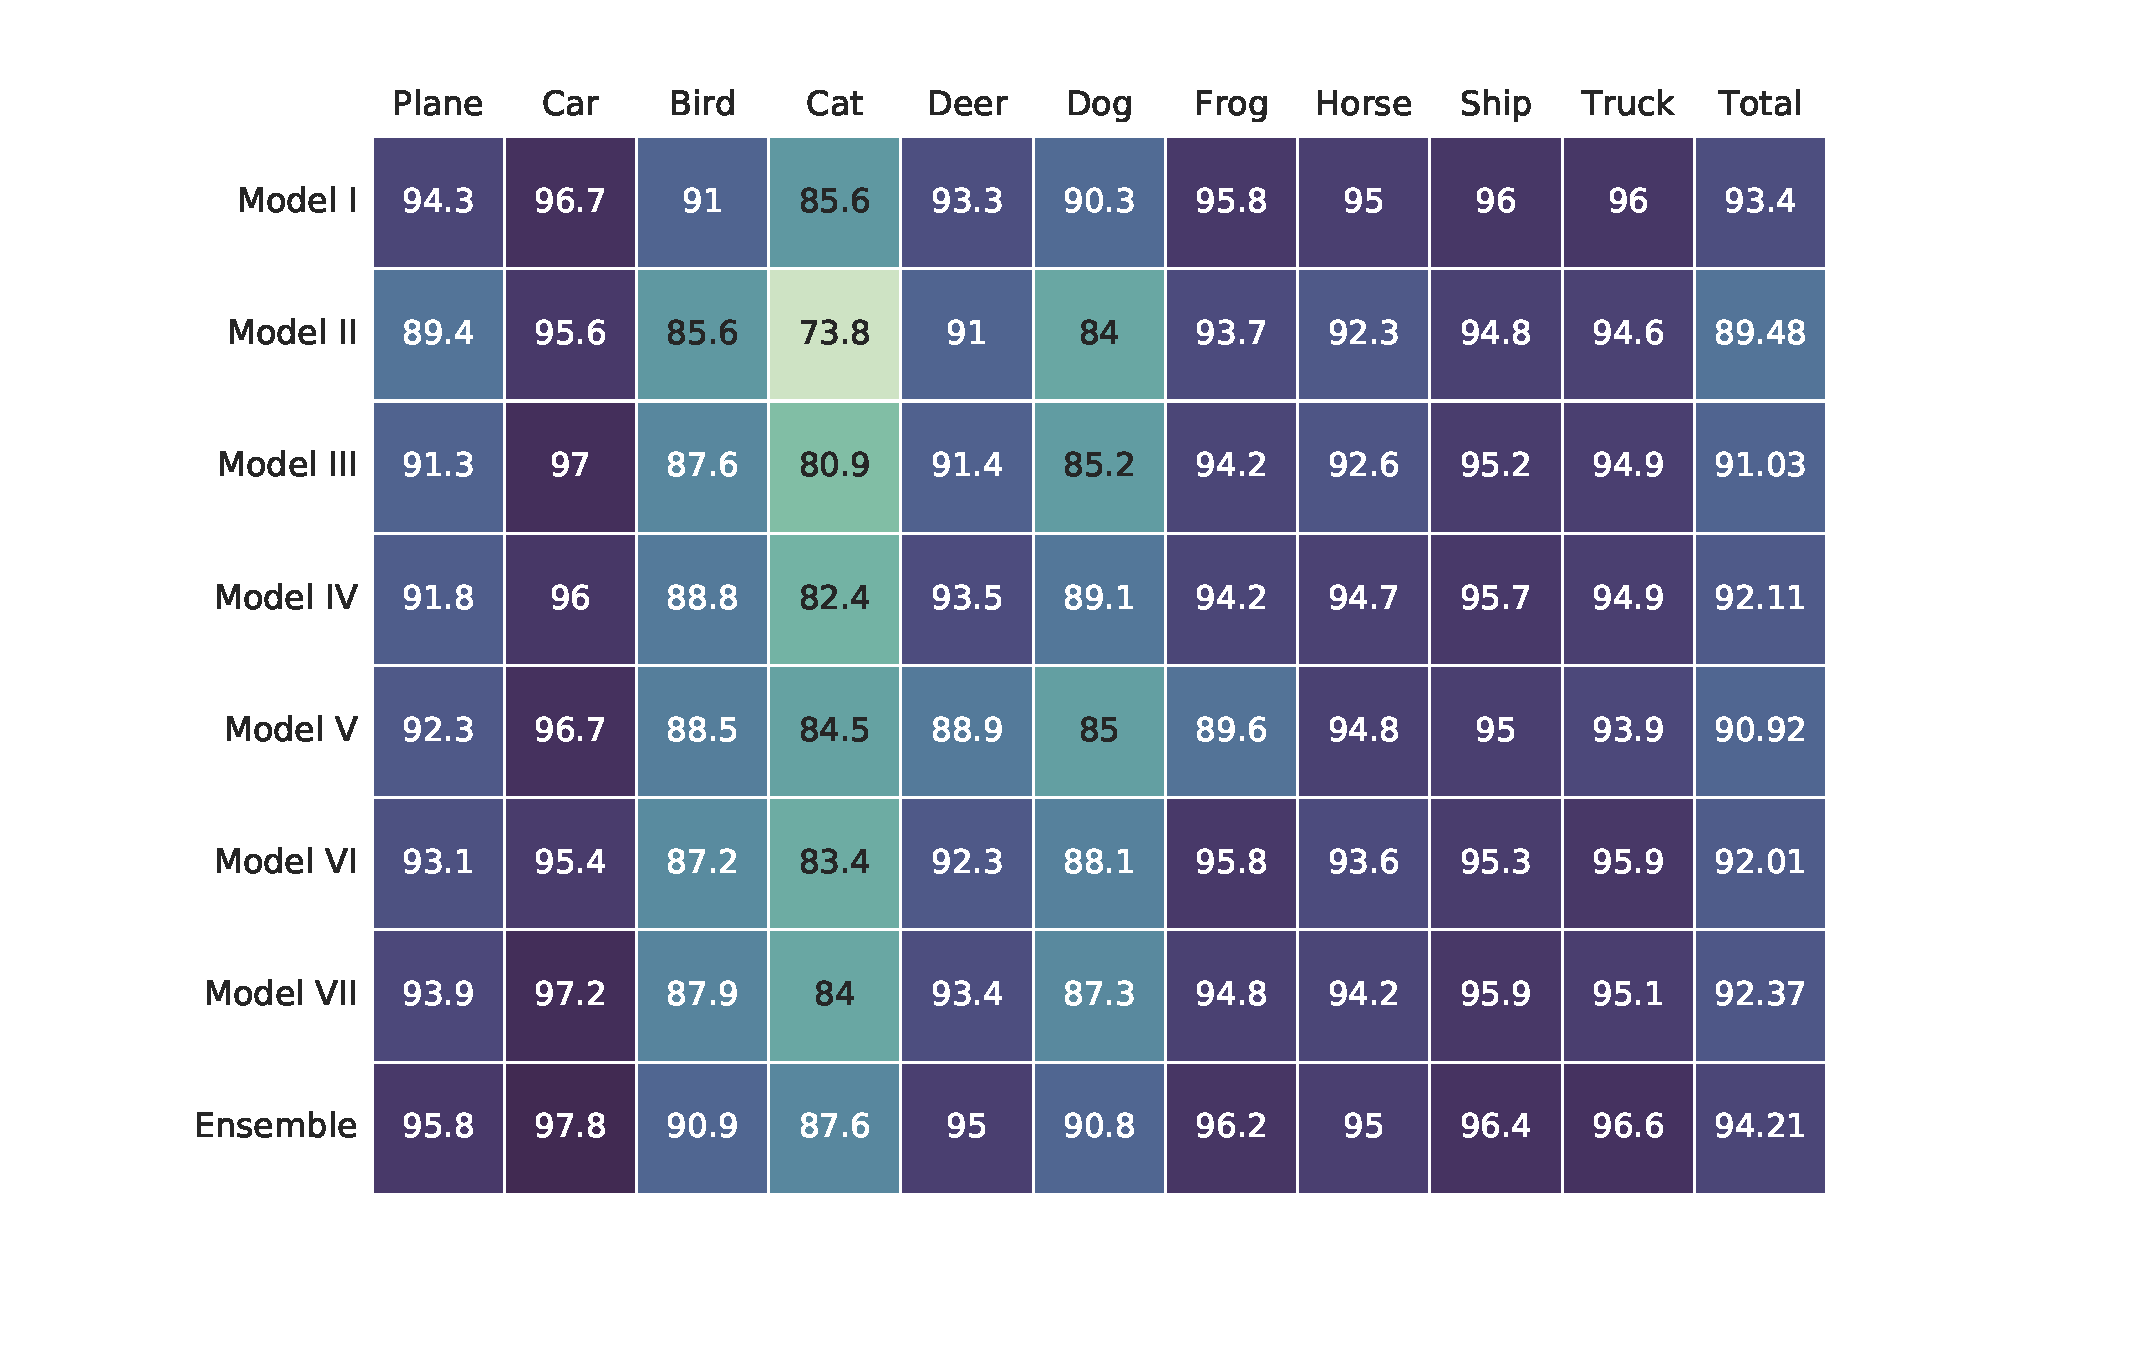
\includegraphics[width=\textwidth]{accuracy_table}
    \vspace*{-2cm}
    \caption{Точности распознавания по различным классам}
    \label{table-accuracy}
\end{figure}

\begin{figure}[H]
    \centering
    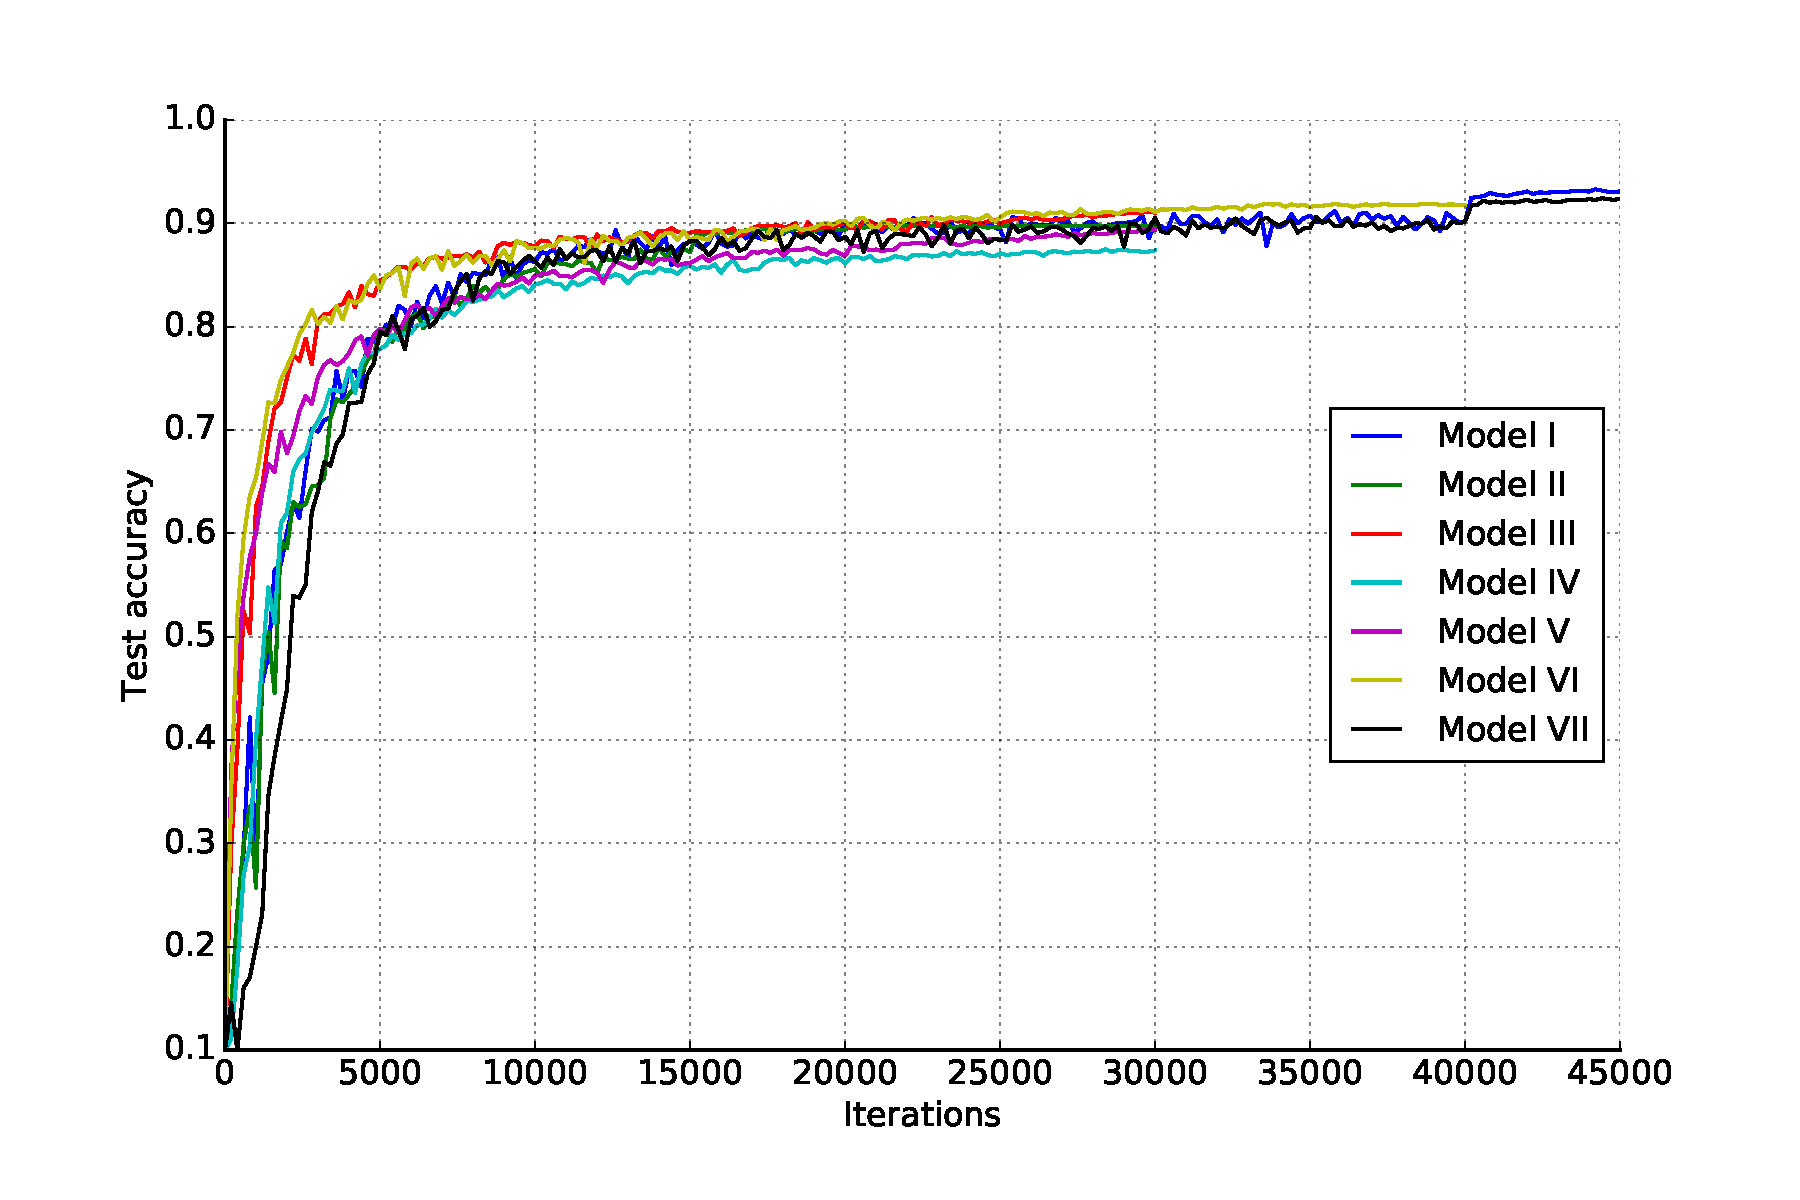
\includegraphics[width=\textwidth]{train_all}
    \vspace*{-1.3cm}
    \caption{Графики обучения моделей}
    \label{fig:train_all}
\end{figure}

\begin{figure}[H]
    \centering
    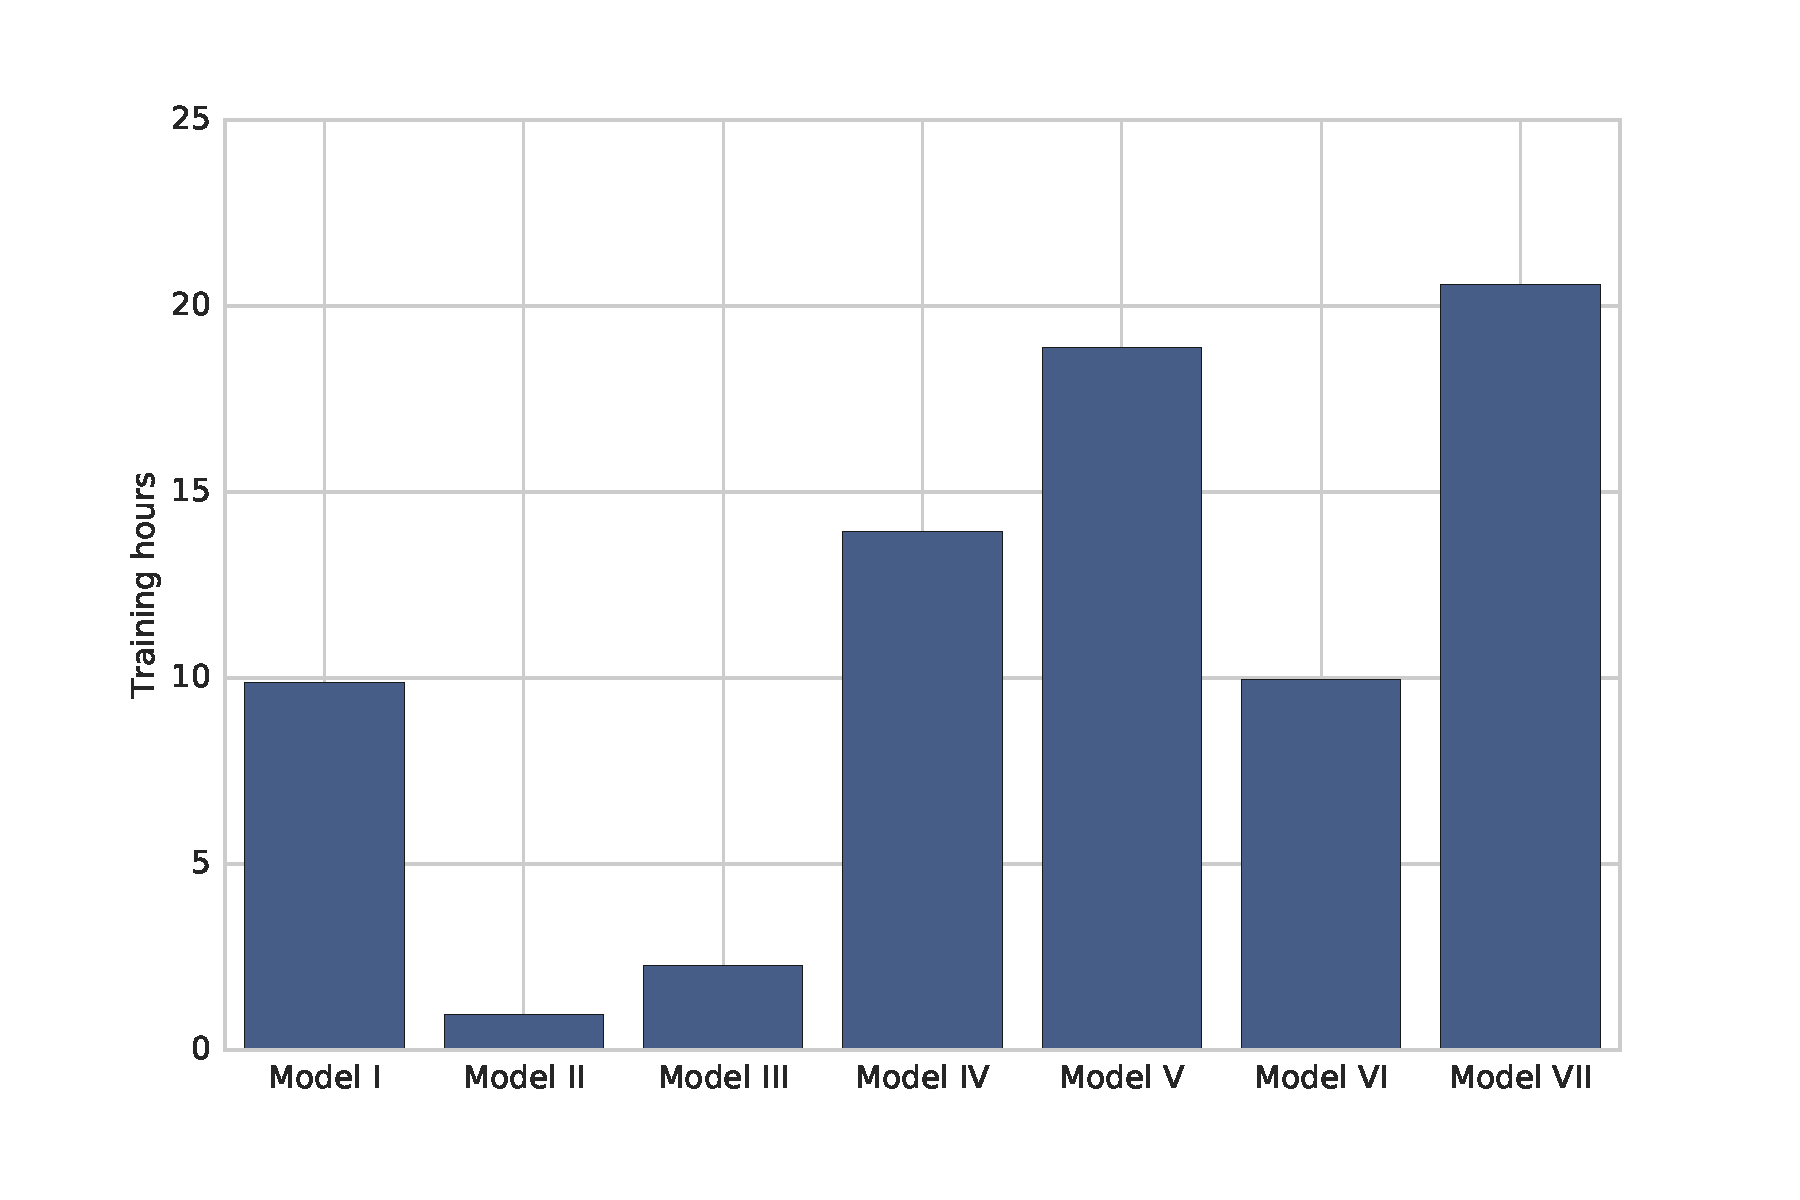
\includegraphics[width=0.9\textwidth]{time_consumption}
    \vspace*{-0.5cm}
    \caption{Время, затраченное моделями на обучение}
    \label{time_consumption}
\end{figure}
\clearpage

\lstinputlisting[language=Python, caption=Препроцессинг изображений]{CIFAR10_zca.py}
\lstinputlisting[language=Python, caption=Оценка модели и запись ответов в таблицу
                                          для дальнейшего построения ансамбля]{predict.py}
\lstinputlisting[language=Python, caption=Построение ансамбля из таблицы ответов нейронных сетей]{ensemble.py} % Приложение
\end{document}